\documentclass[9pt, compress, xcolor=table]{beamer}


\usetheme{m}

\usepackage{amsmath,amssymb}
\usepackage{booktabs}
\usepackage[scale=2]{ccicons}
\usepackage{minted}
% \usepackage[utf8]{inputenc}
% \usepackage[T2A]{fontenc}
% \usepackage[english, russian]{babel}
%%% For accessing system, OTF and TTF fonts
%%% (would have been loaded by polylossia anyway)
\usepackage{fontspec}
%%% For language switching -- like babel, but for xelatex
\usepackage{polyglossia}
% \setmainfont{PT Sans} % вообще шрифты определяются в теме бимера
% заменим на шрифт, доступный в Overleaf
% https://www.overleaf.com/learn/latex/Questions/I_have_a_custom_font_I%27d_like_to_load_to_my_document._How_can_I_do_this%3F
% \setmainfont{[./fonts/FiraSans-Regular.ttf]}
% \setmainfont{Noto Sans}
\setmainlanguage{russian}
\setotherlanguages{english} %% or other languages

\usepackage{graphicx}
\usepackage{tabu} % https://ru.sharelatex.com/learn/Tables
\DeclareGraphicsExtensions{.pdf,.jpg,.png}
\graphicspath{{../images/}{./images/}}

\colorlet{Mycolor1}{green!50!blue!50!}

\usemintedstyle{trac}

\title{Физические принципы микроскопии сверхвысокого разрешения}
\subtitle{осенний семестр, 2016}
\author{ассистент, к.ф.-м.н. Шутова О.А.}
\institute{МГУ им. М.В. Ломоносова, физический факультет}

\begin{document}

\maketitle

\plain{}{Лекция 1. Введение в курс}

\begin{frame}[fragile]
  \frametitle{}
  
Явления, кроме оптических, используемые для построения изображений невидимых невооруженным глазом объектов 
\begin{columns}[c]

\column{6cm}
\begin{figure}
\centering
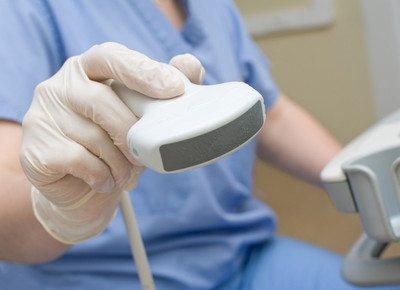
\includegraphics[width=0.75\textwidth]{usi}
\\ \small{Ультразвук}
\end{figure}
\begin{figure}
\centering
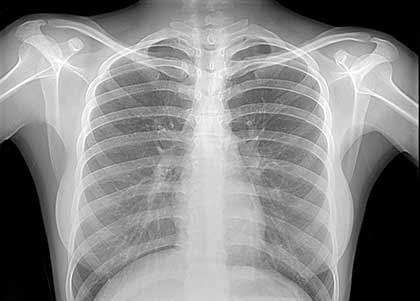
\includegraphics[width=0.75\textwidth]{xray}
\\ \small{Высокочастотное ЭМ (рентген)}
\end{figure}

\column{6cm}

\begin{figure}
\centering
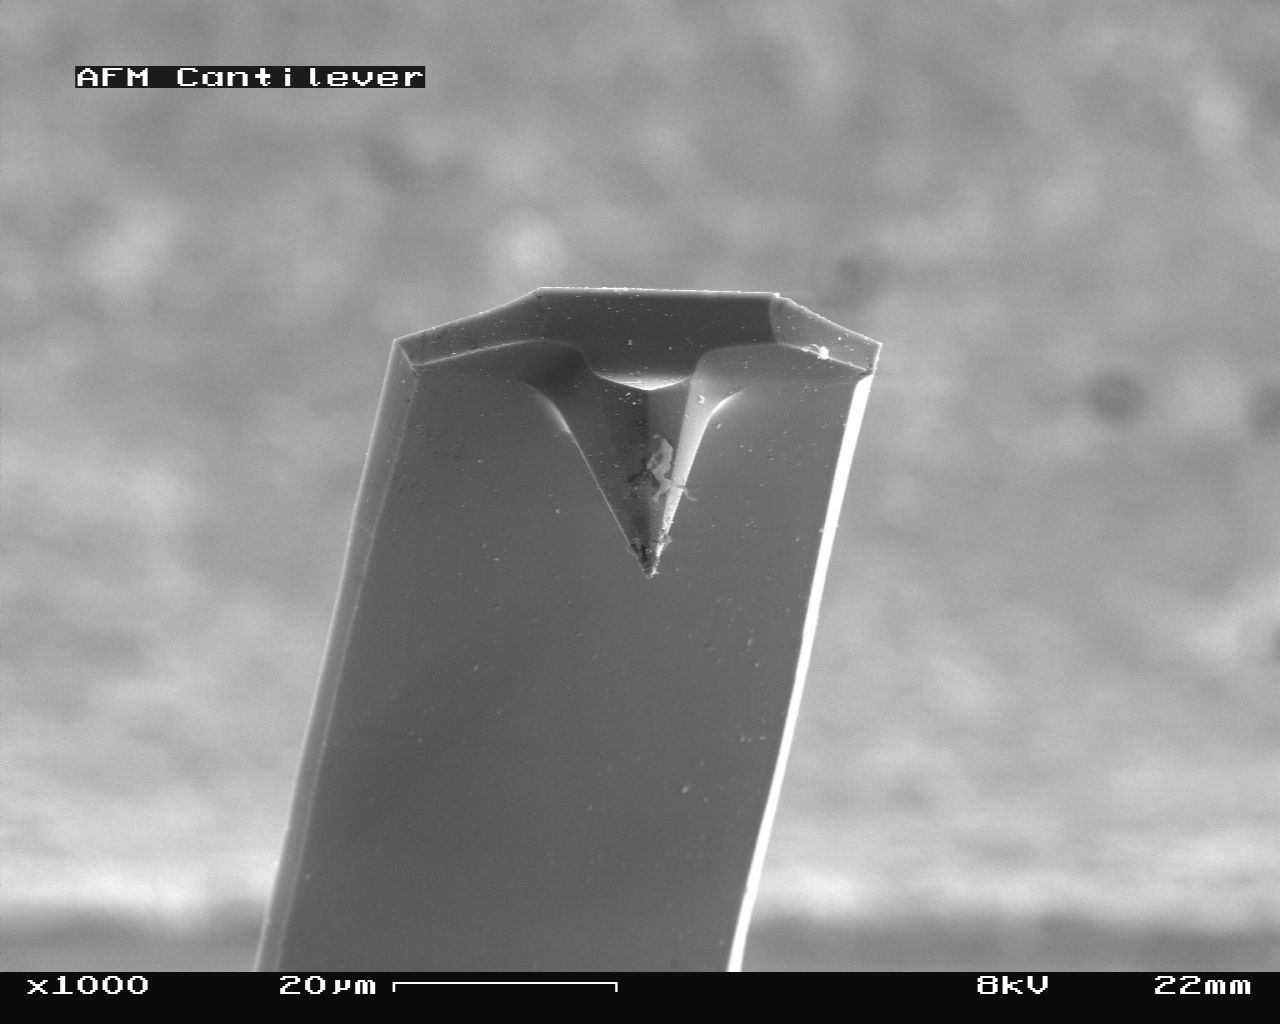
\includegraphics[width=0.75\textwidth]{afm}
\\ \small{Силы Ван-дер-Ваальса (и др. дальнодействующие, shear-force, АСМ, СТМ)}
\end{figure}
\begin{figure}
\centering
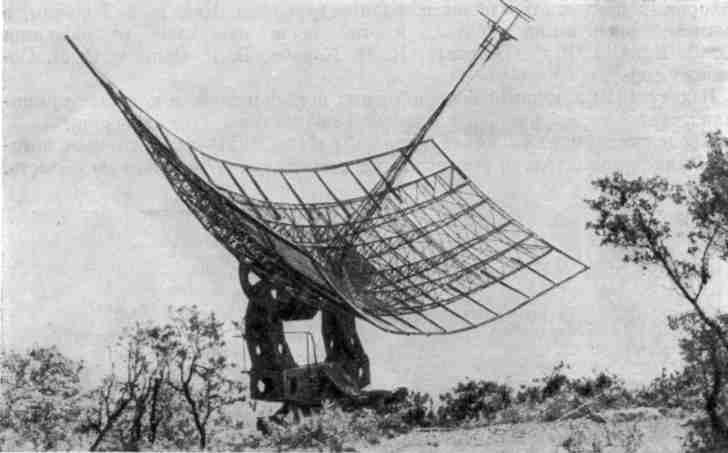
\includegraphics[width=0.75\textwidth]{radio}
\\ \small{Низкочастотное ЭМ (радио)}
\end{figure}

\end{columns}
\end{frame}

\begin{frame}{Свойства электромагнитного излучения оптического диапазона}

\begin{itemize}
    \item \small{Электромагнитное излучение оптического диапазона, локализованного в области чувствительности глаза человека, исходно дано для построения изображений и этим обусловлена его уникальность.}
    
    \item \small{Электромагнитное излучение оптического диапазона не разрушает биологические объекты, с которыми взаимодействует, однако, сильно рассеивается в них.}
    
    \item \small{Находится в области плазмонного резонанса многих металлов.}
    
    \item \small{Имея длину волны порядка сотен нанометров, играет ключевую роль в управлении веществом на нанометровом масштабе, в т.ч. в медицинских приложениях (определение законов развития раковых опухолей и других болезней, транспорт лекарств к опухоли и др.); в хранении и передаче информации; в исследовании физических явлений на этих масштабах.}
    
\end{itemize}

\begin{figure}
\centering
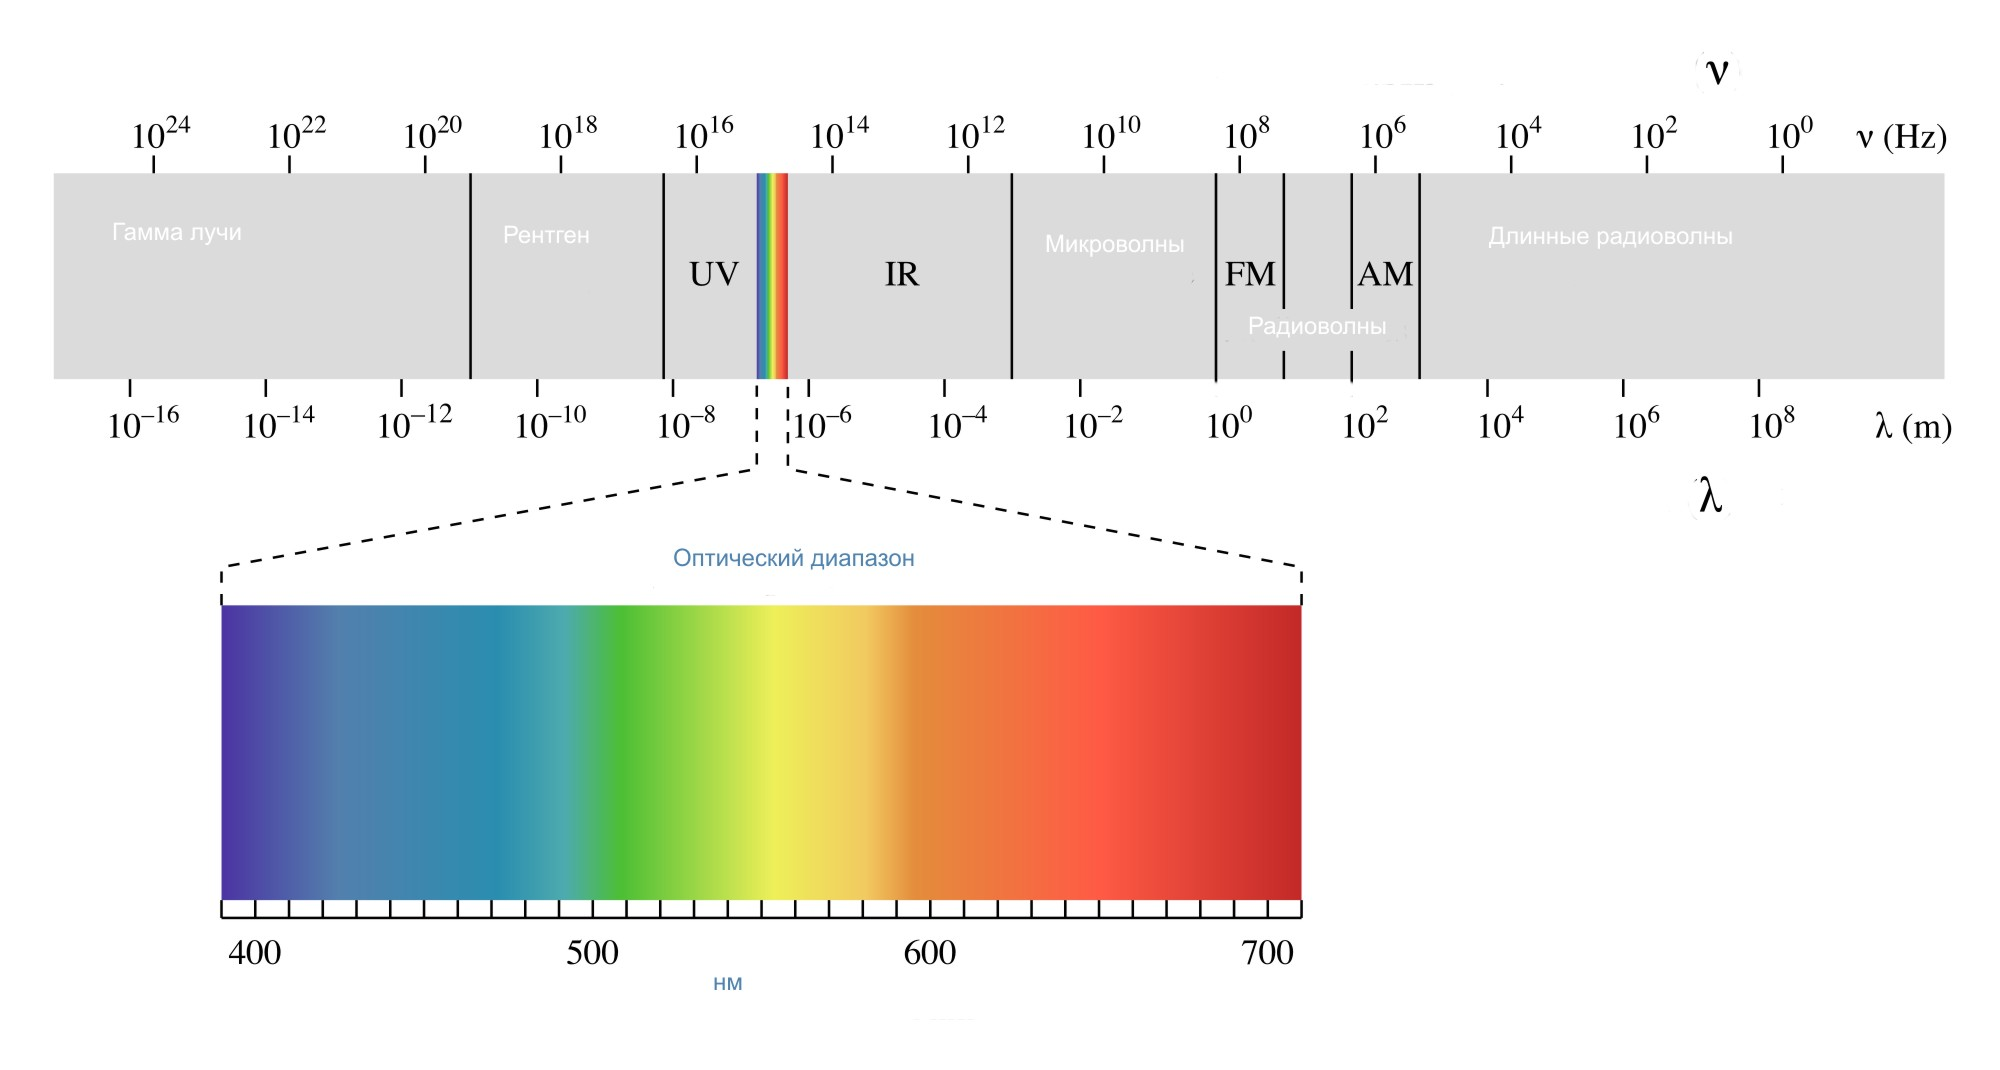
\includegraphics[width=0.7\textwidth]{EM_spectrum}
\end{figure}

\end{frame}

\section{Исторические вехи в оптической микроскопии}

\begin{frame}[fragile]
  \frametitle{1595 г.\,--\,1911 г.}
  
\begin{table}[htbp]
\begin{center}
\small
\arrayrulewidth=1pt
\begin{tabular}{|l|p{.42\textwidth}|p{.4\textwidth}|}
% \begin{tabu} to 0.9\textwidth { | X[l] | X[l] | X[l] | }
% http://tex.stackexchange.com/questions/41758/how-can-i-reproduce-this-table-with-thick-lines
% \begin{tabu}{|l|p{.42\textwidth}|p{.4\textwidth}|}
\hline
\cellcolor{gray!25}\textbf{Год} & 
\cellcolor{gray!25}\textbf{События и люди} & 
\cellcolor{gray!25}\textbf{Объект, разрешающая способность} \\ \hline
\textbf{1595} & 
Изобретение однолинзового микроскопа, Г.~Янсен, А.~фон~Левенгук, Роберт Гук & 
Насекомые, клетка растения; несколько микрон \\ \hline
\textbf{1858} & 
Первое гистологическое окрашивание, Йозеф фон Герлах & 
Ядро клетки мозга, 1 микрон, хороший контраст \\ \hline
 \textbf{1873} & 
Формулировка дифракционного предела визуализации, Эрнст Аббе, лорд Рэлей & Для видимого диапазона~--- не~меньше доли микрон \\ \hline
\textbf{1880} & 
Наилучший традиционный микроскоп с объективом, конденсором, коррекцией аберраций, механикой, Карл Цейсс и Эрнст Аббе & 
Бактерии (туберкулез, чума, сибирская язва); доли микрон \\ \hline
\textbf{1911} & 
Флуоресцентный микроскоп, Макс Хайтингер & 
Разрешение не~улучшается, улучшается лишь качество картинки из-за разного химического сродства частей образца с флуорофором \\ \hline
\end{tabular}\label{tab1}
%\end{tabu}\label{tab1}
\end{center}
\end{table}

\end{frame}

\begin{frame}[fragile]
  \frametitle{1911 г. - 1976 г.}
  
\begin{table}[htbp]
\begin{center}
\small
\arrayrulewidth=1pt
\begin{tabular}{|l|p{.42\textwidth}|p{.4\textwidth}|}
%\begin{tabu} to 0.9\textwidth { | X[l] | X[l] | X[l] | }
% http://tex.stackexchange.com/questions/41758/how-can-i-reproduce-this-table-with-thick-lines
%\begin{tabu}{|l|p{.42\textwidth}|p{.4\textwidth}|}
\hline
\cellcolor{gray!25}\textbf{Год} & 
\cellcolor{gray!25}\textbf{События и люди} & 
\cellcolor{gray!25}\textbf{Объект, разрешающая способность} \\ \hline
\textbf{1935} & 
Метод фазового контраста, Фритц Цернике & 
Без использования красителя увидеть прозрачные биологические объекты \\ \hline
\textbf{1939} & 
Поляризационная микроскопия, В. Шмидт, Шинья Иноуэ & 
Внутреннее строение клетки, процесс деления живой клетки \\ \hline
\textbf{1955} & 
Диференциально"=интерференционная микроскопия или микроскопия по Номарскому, Ежи Номарский & 
Транспорт мембранной везикулы вдоль нейронного отростка, 50-100 нм (удалось подавить гало в методе ФК) \\ \hline
\textbf{1961} & 
Концепция конфокальной микроскопии, Марвин Минский& 
Эндоплазматическая сеть клеток плазмоцитомы (онкология крови) \\ \hline
\textbf{1976} & 
FRET: микроскопия на основе фёрстеровского переноса энергии, Т.~Фёрстер, Т.~Йовин & 
Взаимодействие белков внутри клетки \\ \hline
\end{tabular}\label{tab2}
%\end{tabu}\label{tab1}
\end{center}
\end{table}

\end{frame}

\begin{frame}[fragile]
  \frametitle{1976 г. - 1994 г.}
  
\begin{table}[htbp]
\begin{center}
\small
\arrayrulewidth=1pt
\begin{tabular}{|l|p{.42\textwidth}|p{.4\textwidth}|}
%\begin{tabu} to 0.9\textwidth { | X[l] | X[l] | X[l] | }
% http://tex.stackexchange.com/questions/41758/how-can-i-reproduce-this-table-with-thick-lines
%\begin{tabu}{|l|p{.42\textwidth}|p{.4\textwidth}|}
\hline
\cellcolor{gray!25}\textbf{Год} & 
\cellcolor{gray!25}\textbf{События и люди} & 
\cellcolor{gray!25}\textbf{Объект, разрешающая способность} \\ \hline
\textbf{1981} & 
TIRF: флуоресцентная микроскопия на основе ПВО, Даниэль Аксельрод & 
Процессы в клеточной мембране, ионный транспорт и др. \\ \hline
\textbf{1990} & 
Двухфотонная микроскопия, Мария Гёпперт-Майер, Поль Денк & 
Хромосомы в живых клетках, динамика кальция в пирамидальных нейронах мозга живых мышей. Сигнал флуоресценции гораздо меньше, не вредит живому организму, объем области сигнала тоже гораздо меньше~--- разрешение \\ \hline
\textbf{1993} & 
SNOM: ближнепольный сканирующий оптический микроскоп, Эрик Бетциг, Роберт Чичестер& 
Начало расшифровки ДНК, новое видение внутриклеточных процессов \\ \hline
\textbf{1994} & 
GFP~--- зеленый флуоресцентный белок, Aequorea victoria (медуза), Осаму Шимонура, Мартин Чалфи, Роджер Тсин& Белковая динамика в живых клетках  \\ \hline
\end{tabular}\label{tab3}
%\end{tabu}\label{tab1}
\end{center}
\end{table}

\end{frame}


\begin{frame}[fragile]
  \frametitle{Преодоление дифракционного предела}
  
\begin{table}[htbp]
\begin{center}
\small
\arrayrulewidth=1pt
\begin{tabular}{|l|p{.42\textwidth}|p{.4\textwidth}|}
%\begin{tabu} to 0.9\textwidth { | X[l] | X[l] | X[l] | }
% http://tex.stackexchange.com/questions/41758/how-can-i-reproduce-this-table-with-thick-lines
%\begin{tabu}{|l|p{.42\textwidth}|p{.4\textwidth}|}
\hline
\cellcolor{gray!25}\textbf{Год} & 
\cellcolor{gray!25}\textbf{События и люди} & 
\cellcolor{gray!25}\textbf{Объект, разрешающая способность} \\ \hline
\textbf{2000} & 
STED~--- микроскопия на основе истощения накачки + SIM~---структурирование возбуждающего поля, Штефан Хель &
Кубит (азот-вакантный центр в алмазе), прорыв от сотен до долей нанометров \\ \hline
\textbf{2002} & 
PA-GFP~--- фотоактивируемый зеленый флуоресцентный белок, Сергей Лукьянов& Динамика белкового взаимодействия \\ \hline
\textbf{2006} &
PALM/STORM~--- микроскопия на основе фотоактивируемой локализации, Э.~Бетциг &
Десятки нанометров \\ \hline
\end{tabular}\label{tab4}
%\end{tabu}\label{tab1}
\end{center}
\end{table}
\begin{figure}
\centering
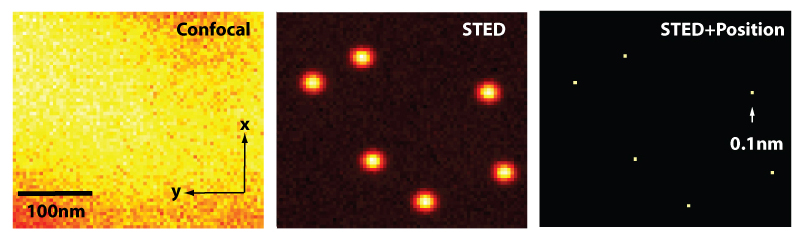
\includegraphics[width=0.6\textwidth]{diamond-stedL}
\\ Изображение азот-вакантного центра (для кубитов)
\end{figure}

\end{frame}


\section{Предел разрешения в классическую эпоху}
\begin{frame}[fragile]
  \frametitle{1595 г. - изобретение первого микроскопа}
\begin{columns}[c]
\column{6cm}
\begin{figure}
\centering
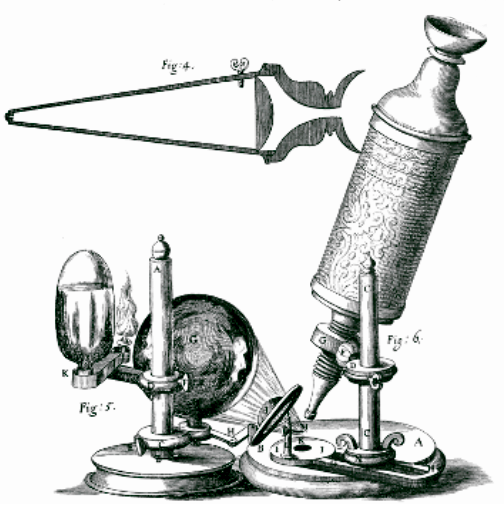
\includegraphics[width=0.7\textwidth]{microscope}
\\ Рисунок руки Роберта Гука
\end{figure}
Первое упоминание о микроскопе относится к 1595 г. В письме датского посланника французского суда У. Бореля сказано о мастере по очкам Гансе Янсене и его сыне Захарии. 
\column{6cm}
\begin{figure}
\centering
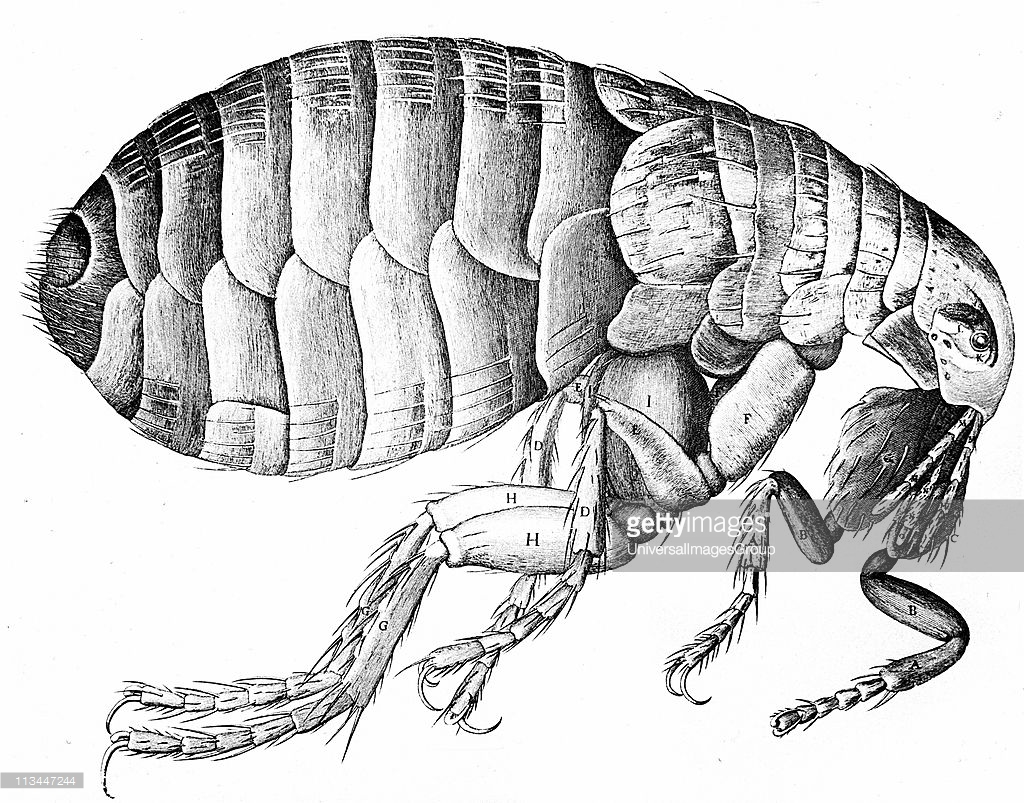
\includegraphics[width=0.7\textwidth]{flea}
\\ Из книги Роберта Гука \emph{Micrographia} 
\newline (1665 г.)
\end{figure}
Хотя официальным родоночальником микроскопа считается Антони ван Левенгук, но это уже было веком позже. Впрочем, за свою жизнь ван Левенгук сделал более полутысячи микроскопов.
\end{columns}
\end{frame}

\begin{frame}[fragile]\frametitle{Ход лучей в классическом микроскопе}
\begin{figure}
\centering
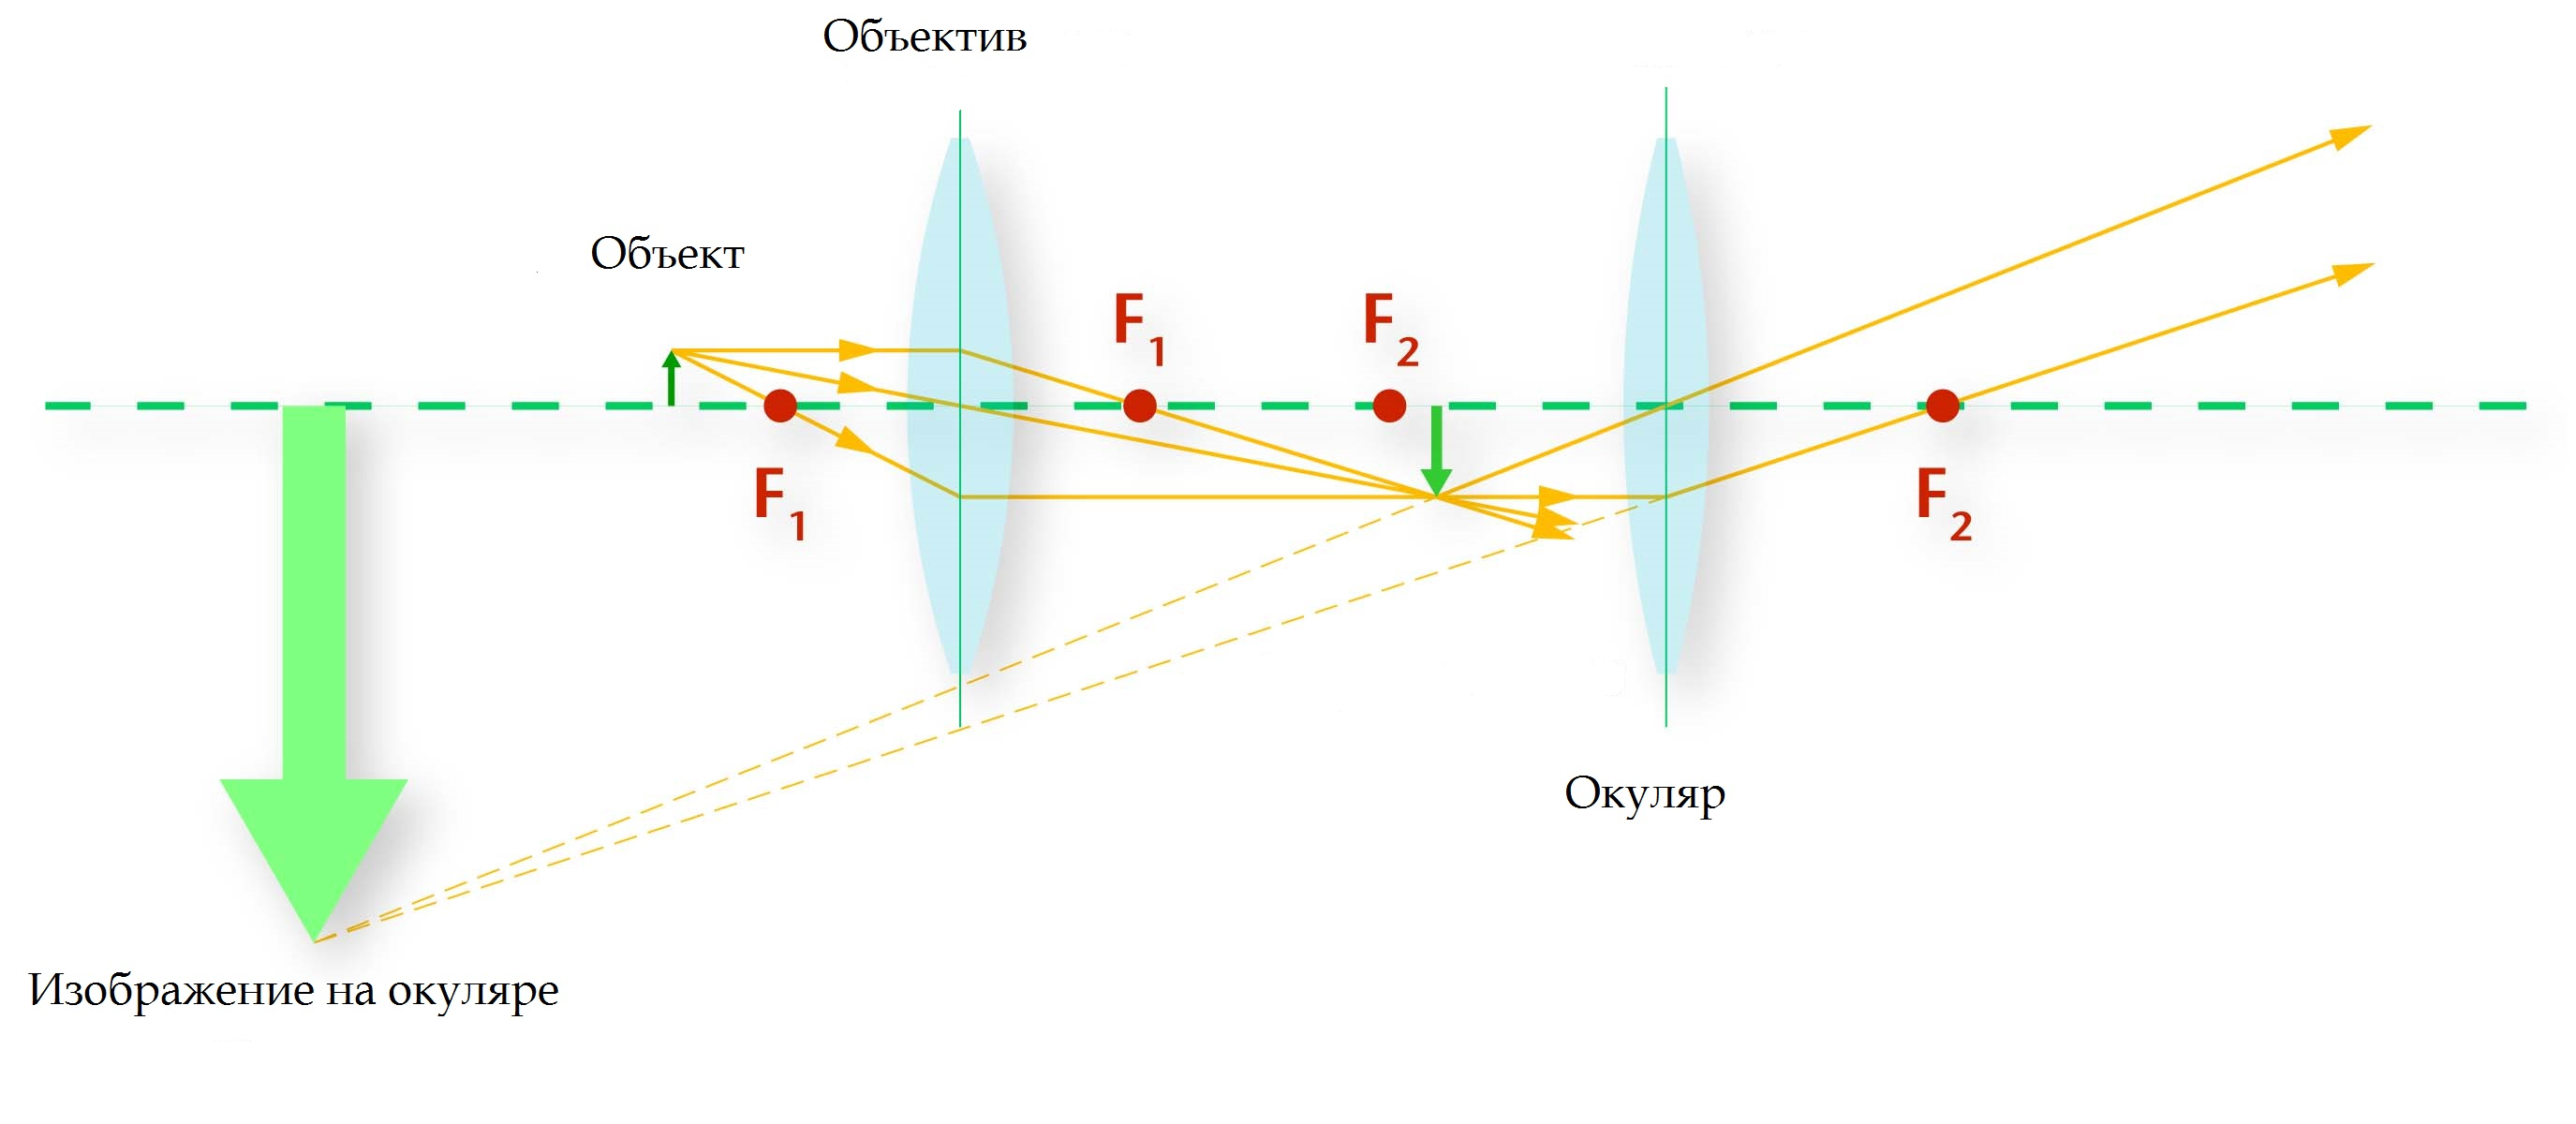
\includegraphics[width=11cm]{Microscope2}
\end{figure}
Для характеристики качества линзы вводится понятие \textcolor{red}{числовой апертуры}, равной $NA=n sin \theta_{max}$ (для воздуха $n=1$).

Самые лучшие доступные коммерчески линзы имеют $NA=1.4$, это так называевые иммерсионные объективы (для иммерсионного масла $n=1.5$).
\end{frame}

\begin{frame}[fragile]\frametitle{Принцип действия иммерсионного объектива}
\textcolor{Mycolor1}{Маслянный иммерсионный объектив:}

\begin{columns}[c]
\column{8cm}

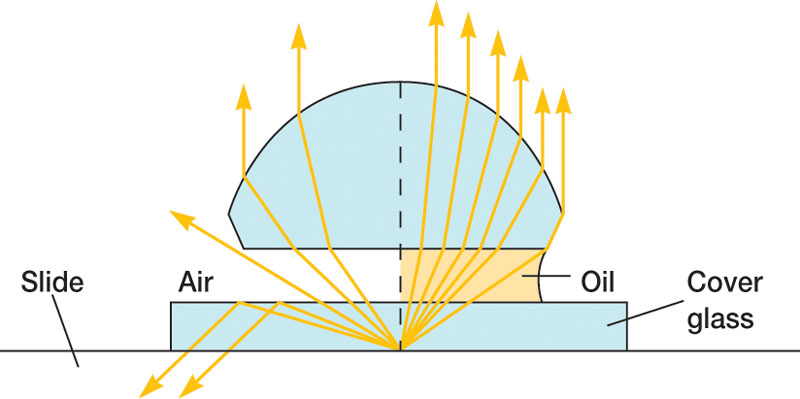
\includegraphics[width=0.9\textwidth]{oil}

\column{4cm}
Обычно используют очищенное кедровое или минеральное масло, можно назвать этот метод методом согласования показателей преломления.

Чтобы понять принцип можно провести такой простой эксперимент:
\end{columns}

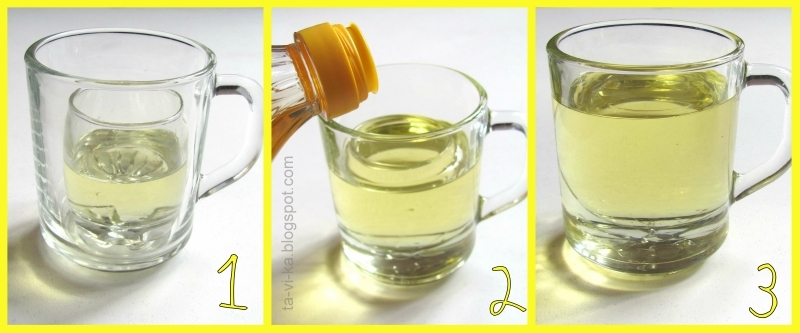
\includegraphics[width=0.8\textwidth]{immerse}

\end{frame}

\begin{frame}[fragile]\frametitle{Принцип действия иммерсионного объектива}
\textcolor{Mycolor1}{Твердотельные иммерсионные объективы:}
\begin{columns}[c]
\column{6cm}
Твердотельные иммерсионные объективы: полусфера и гиперполусфера
\\
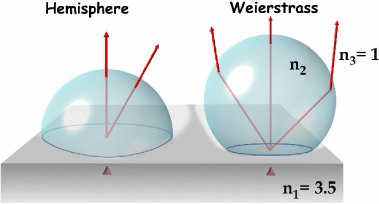
\includegraphics[width=0.9\textwidth]{wl_1}

позволяют гораздо сильнее концентрировать лучи, доводя числовую апертуру до 2.

\column{6cm}
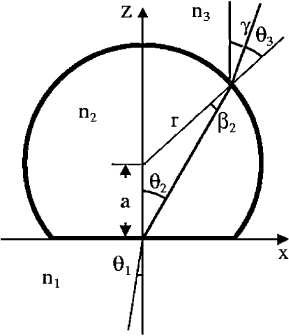
\includegraphics[width=0.9\textwidth]{wl_2}

Геометрия гиперполусферы Вейерштрасса
\end{columns}

\end{frame}

\begin{frame}{Твердотельный иммерсионный объектив}
\centering
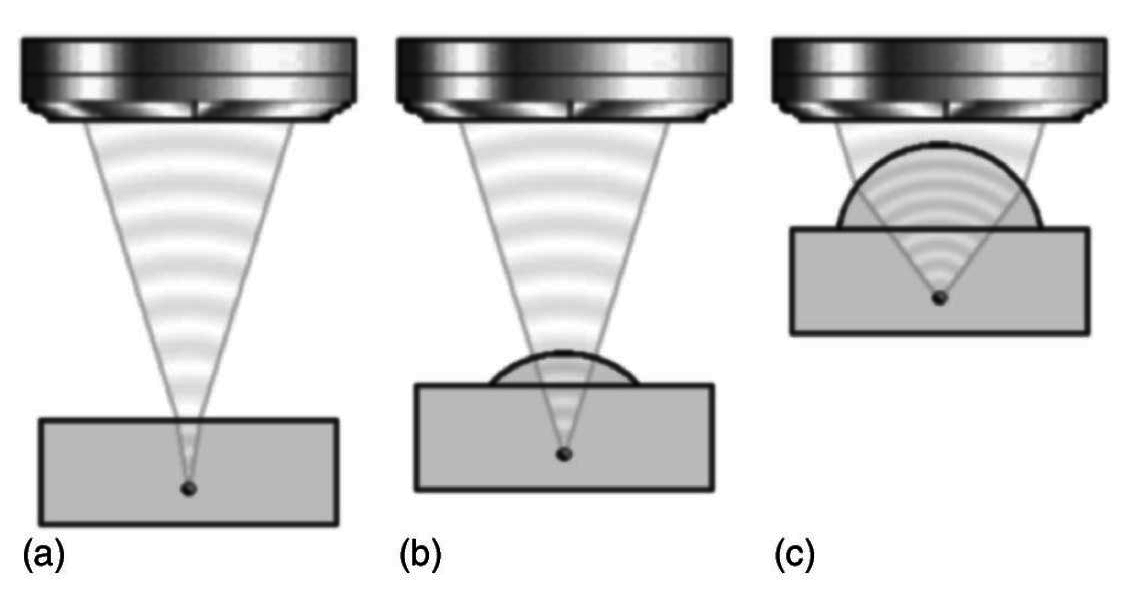
\includegraphics[width=0.9\textwidth]{sio}

Позволяет достичь оптимальной аподизации на небольшом удалении от объекта.
\end{frame}


\begin{frame}[fragile]
  \frametitle{1873 г.~--- дифракционный предел разрешения}
  \begin{columns}[c]
\column{6cm}
\begin{figure}
\centering
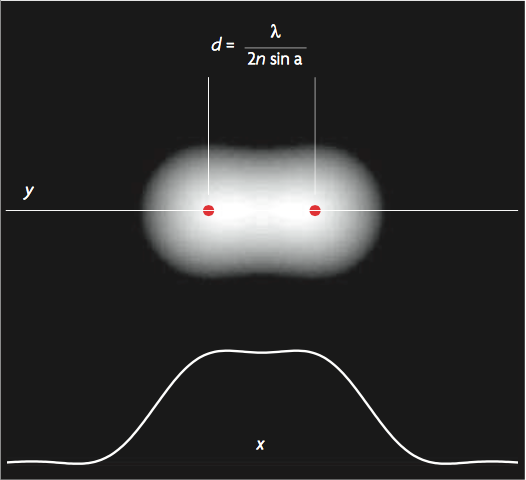
\includegraphics[width=0.7\textwidth]{Abbe}
\\ Дифракционный предел
\end{figure}
 
\column{6cm}
\begin{figure}
\centering
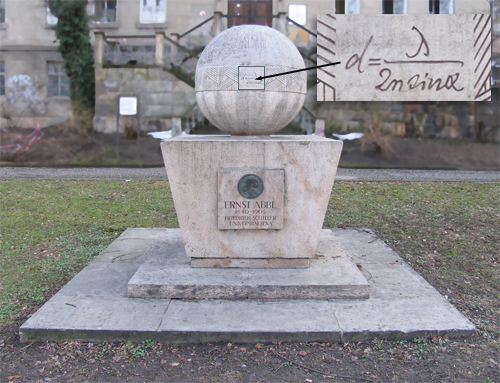
\includegraphics[width=0.7\textwidth]{AbbeEqL}
\\ Формула Аббе в камне
\end{figure}

\end{columns}

Теория разрешения сформулирована \textcolor{red}{Аббе (Ernst
Karl Abbe) в 1873 г. и лордом Рэлеем (Lord Rayleigh John
William Strutt) в 1879 г.} и она утверждает, что предельное
разрешение в визуализации объектов составляет $\frac{\lambda}
{2 n sin \alpha}$.

Так что использование хороших объективов повышает предел разрешения в полтора-два раза.
\end{frame}


\begin{frame}{ДНК --- белок --- клетка}
\begin{columns}[c]

\column{1.7in}
\begin{center}
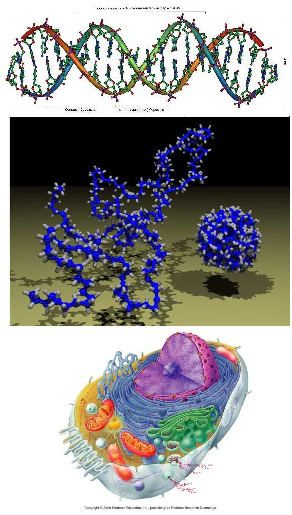
\includegraphics[scale=0.8]{DNA-protein-cell-short}
\end{center}

\column{2.1in}
\begin{block}{Характерные масштабы}

"<Период"> спирали ДНК: \\
$d_{\text{ДНК}}\approx3.4$~нм, \\
Ширина ДНК: \\
$w_{\text{ДНК}}\approx2.2-2.4$~нм, \\
Белковые молекулы:\\
$r_{\text{белок}}\approx1-100$~нм, \\
Ядрышко клетки: \\
$r_{\text{ядрышко}}\approx1-5$~мкм, \\
Ядро клетки: \\
$r_{ядро}\approx5-30$~мкм, \\
Лейкоциты: \\
$r_{лейкоцит}\approx1-4$~мкм.\\
Нервная клетка с отростком: \\
$r_{нервная клетка}<150$~cм.
\end{block}
\end{columns}
\end{frame}

\begin{frame}{CD --- DVD --- Blue-Ray}
\begin{columns}[c]

\column{1.7in}
\begin{center}
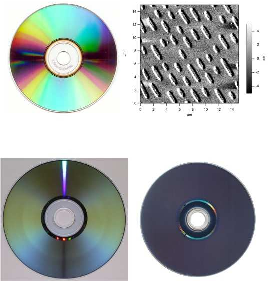
\includegraphics[scale=1.0]{CD-DVD-BlueRay-short}
\end{center}

\column{2.1in}
\begin{block}{Характерные масштабы}

CD ширина пита: \\
$w_{\text{pit}}\approx500$~нм, \\
CD расстояние между питами: \\
$\ell_{\text{pit}}\approx840$~нм, \\
DVD расстояние между питами: \\
$\ell_{\text{DVD}}\approx400$~нм, \\
Blue-ray расстояние между питами: \\
$\ell_{Blue-ray}\approx150$~нм, \\
Blue-ray диаметр пита: \\
$d_{Blue-ray}\approx320$~нм.
\end{block}

\end{columns}
\end{frame}



\begin{frame}{Ядро --- атом --- молекула}

\begin{columns}[c]

\column{1.6in}

\begin{center}
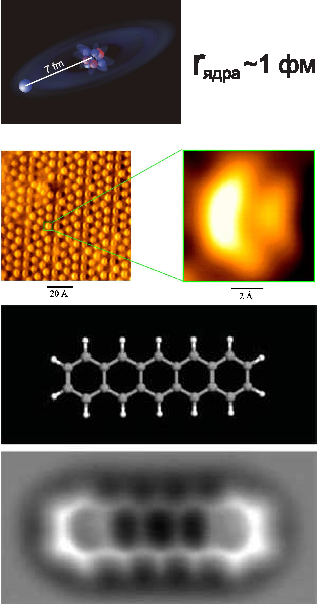
\includegraphics[scale=0.7]{Nucleus-atom-molecula}
\end{center}

\column{2.2in}

\begin{block}{Характерные масштабы}

Радиус ядра H: \\
$r_{\text{H}}\approx10^{-6}$~нм, \\
Радиус атома H: \\
$r_{\text{H}}\approx0.053$~нм, \\
Радиус атома Si: \\
$r_{\text{Si}}\approx0.132$~нм, \\
Радиус молекулы воды: \\
$r_{H_2O}\approx0.25$~нм, \\
Длина молекулы пентацена: \\
$\ell_{C_{22}H_{14}}\approx1.4$~нм.
\end{block}

\end{columns}

\end{frame}


\begin{frame}[fragile]
\frametitle{1935 г.~--- метод фазового контраста}
\begin{figure}
\centering
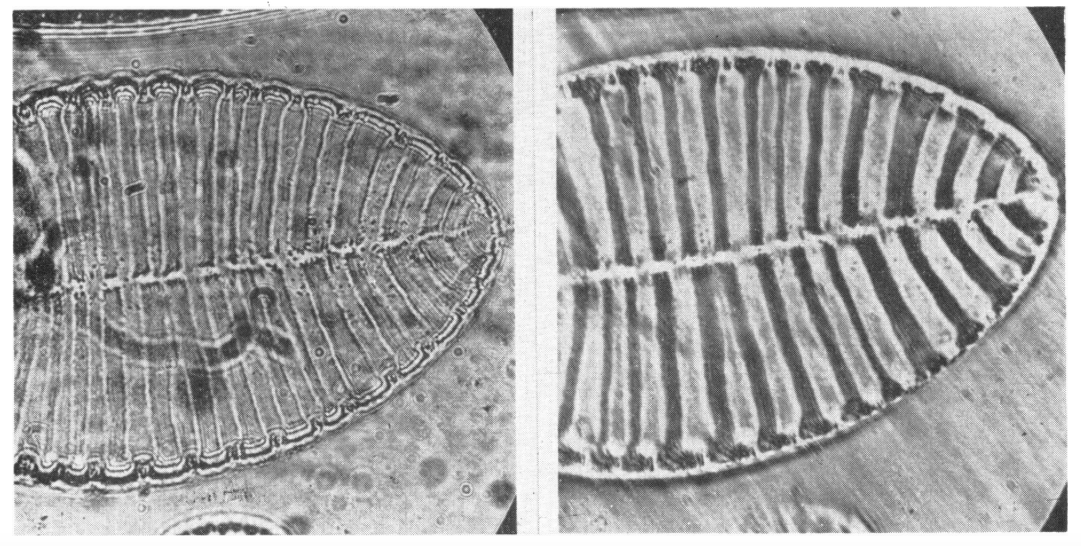
\includegraphics[width=0.9\textwidth]{ph_c}
\\ Изображение без фазового контраста (слева) и с фазовым контрастом (справа)
\end{figure}

\alert{Фритц Цернике}  в 1935 г. предложил метод фазового контраста, за который в 1953 году получил Нобелевскую премию (только через 10 лет после предложения автора фирма Carl Zeiss начала использовать метод Цернике).

\end{frame}

\begin{frame}{Метод фазового контраста Ф. Цернике}
\begin{columns}[c]
\column{8cm}
\begin{center}
\begin{figure}
\centering
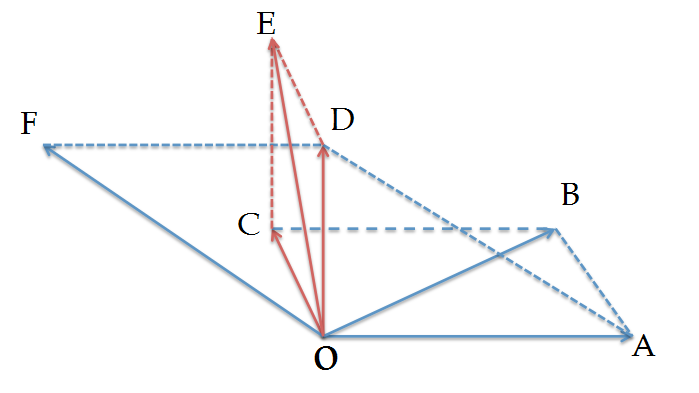
\includegraphics[width=0.9 \textwidth]{phc1}
\\Как  превратить информацию о фазе, увидеть которую мы не можем, в видимую картину интенсивности? (Схема сложения векторов.)
\end{figure}
\end{center}
 
 \column{5cm}
\begin{center}
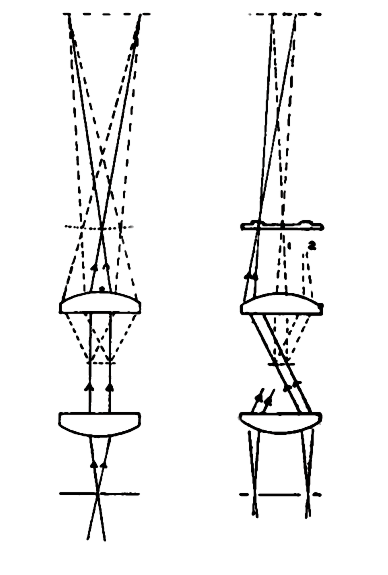
\includegraphics[width=0.9\textwidth]{phc0}
\\{\scriptsize Сравнение двух схем обычной и по методу фазового контраста.}
\end{center}
\end{columns}
\end{frame}

\section{Субволновая оптика}


\begin{frame}{Первое наблюдение эванесцентных волн}

\begin{columns}[c]
\column{6cm}
\begin{center}
\begin{figure}
\centering
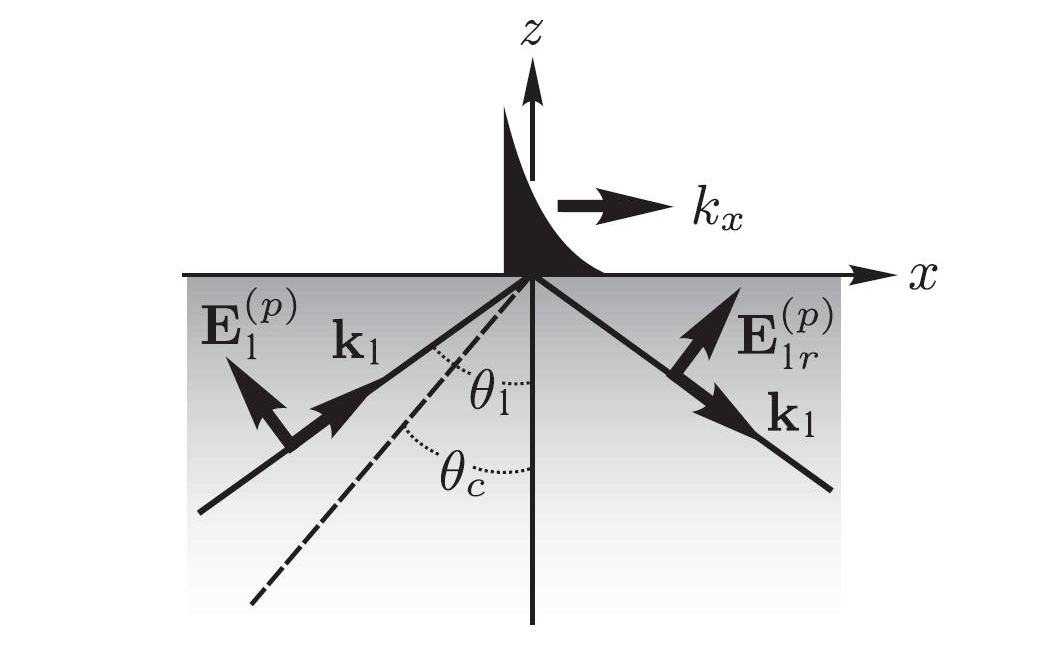
\includegraphics[width=0.9 \textwidth]{ew}
\\Эванесцентная (букв. исчезающая, в русск. литературе ранее~--- неоднородная) волна
\end{figure}
\end{center}
 
 \column{6cm}
\begin{center}
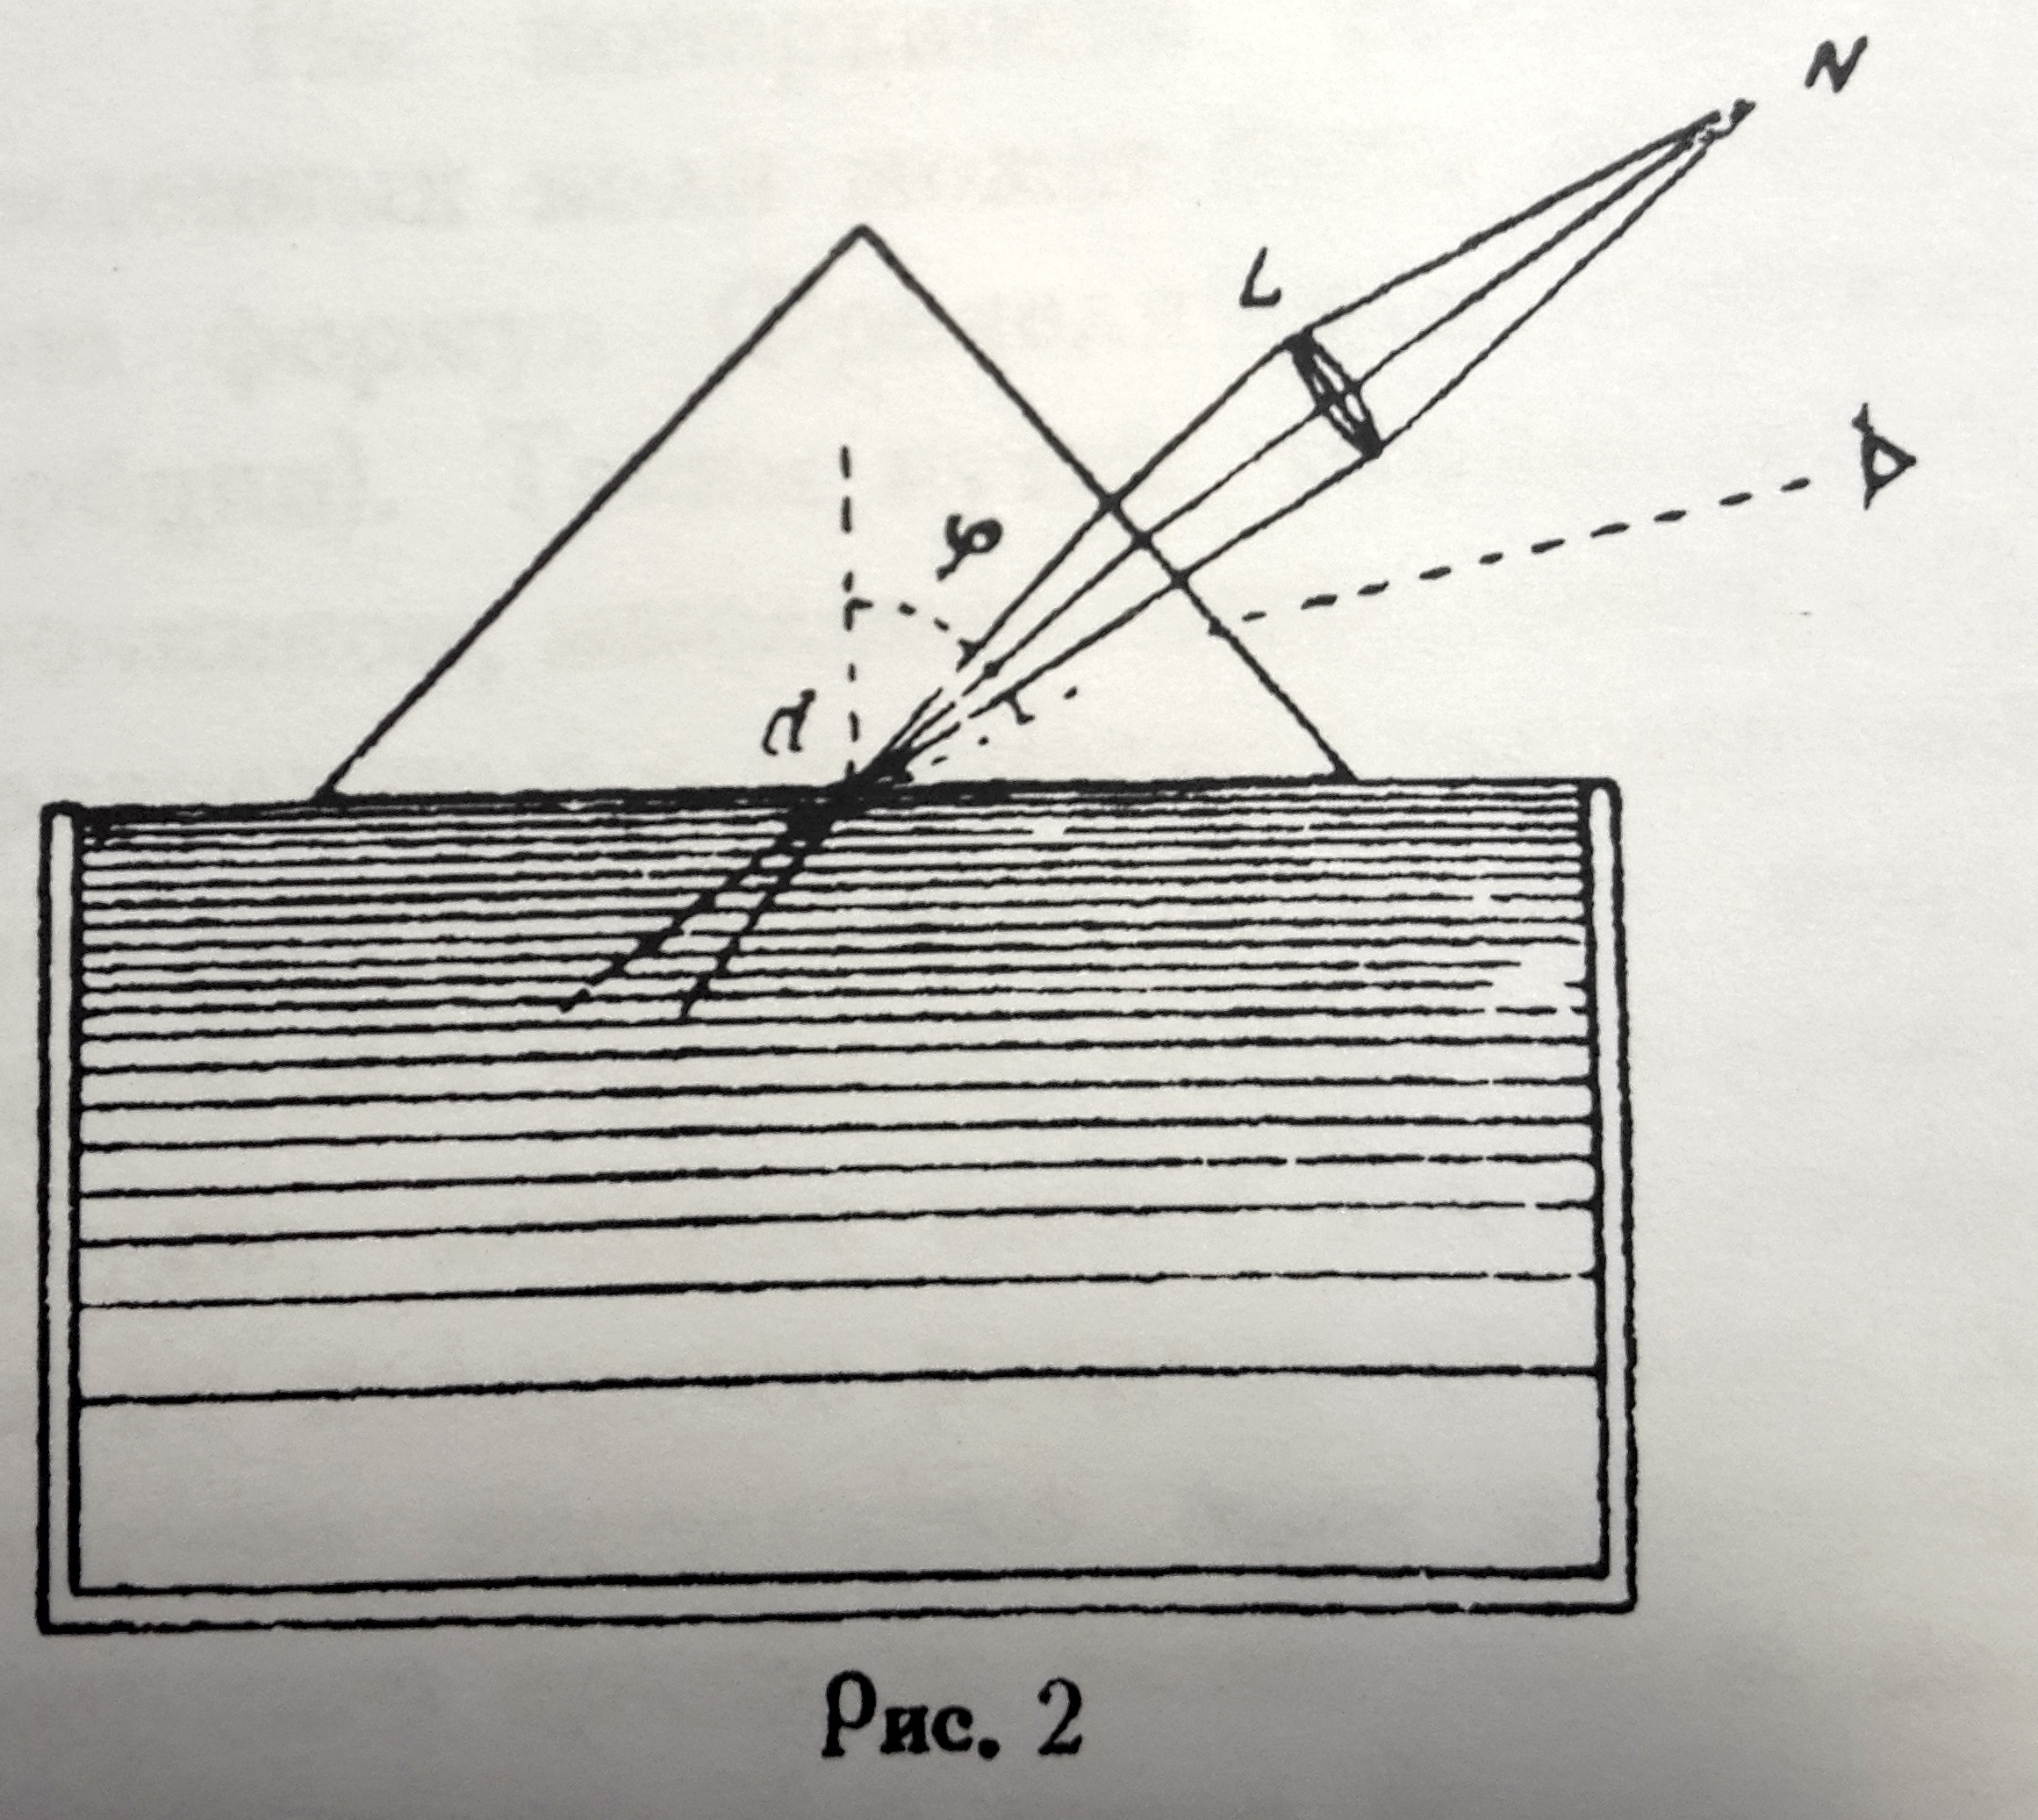
\includegraphics[width=0.9\textwidth]{mand2}
\end{center}
\end{columns}

\begin{block} 

Впервые описана в работе Л.И. Мандельштама "<Излучение источника света, находящегося очень близко от границы раздела двух прозрачных сред">, 1914 г.

\end{block}

\end{frame}

\begin{frame}{Зачем она нам нужна, если она затухает?}
Вспомним, что такое полное внутреннее отражение:

\begin{columns}[c]
\column{6.5cm}
\begin{center}
\begin{figure}
\centering
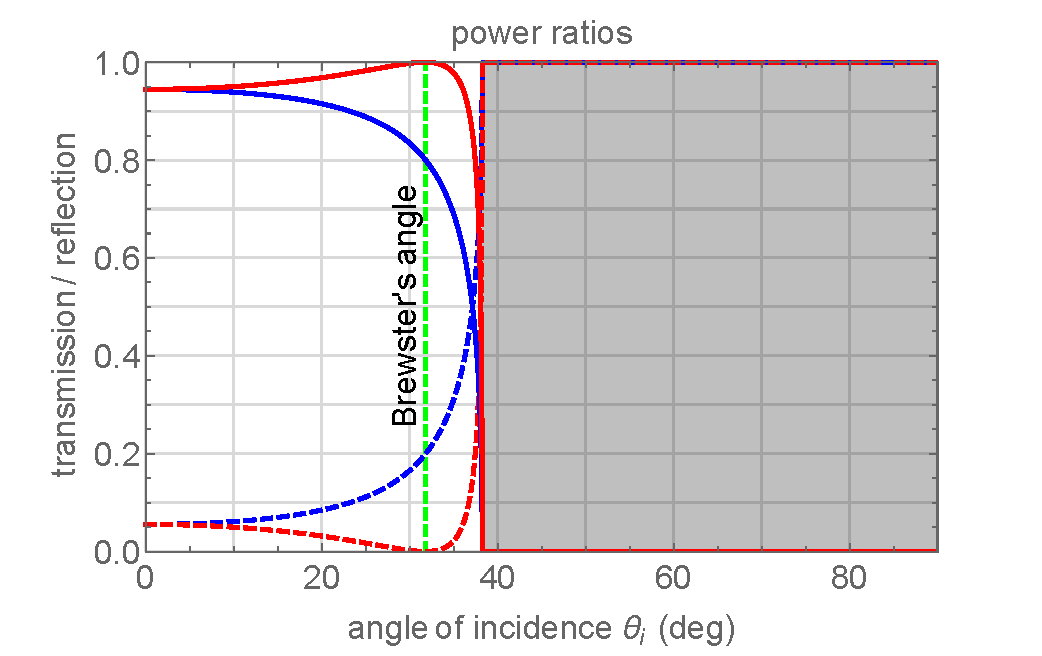
\includegraphics[width=0.9 \textwidth]{fc_p}
\\\scriptsize{Отношение интенсивностей прошедших и отраженных волн и падающей волны}
\end{figure}
\end{center}
 
 \column{6.5cm}
\begin{center}
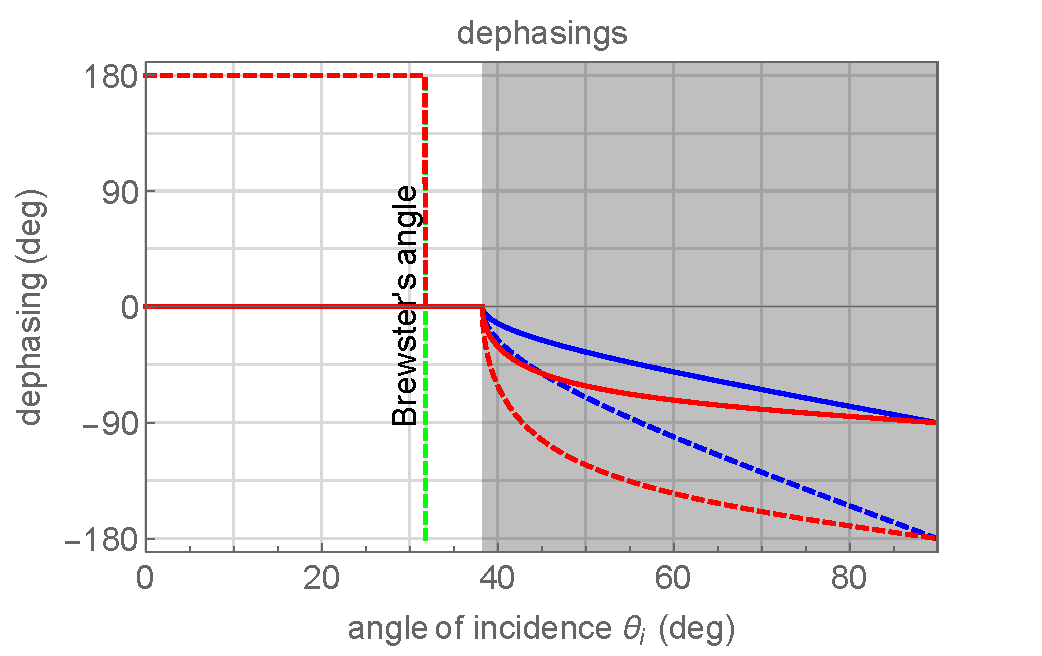
\includegraphics[width=0.9\textwidth]{fc_d}
\\\scriptsize{Отношение фазового сдвига прошедших и отраженных волн с падающей волной}
\end{center}
\end{columns}

В силу непрерывности тангенциальной компоненты волнового вектора, когда мы оказываемся в области ПВО и волновой вектор среды прохождения оказывается мал, должно быть нечто, что обеспечит нам эту непрерывность, это и есть эванесцентная волна!


\end{frame}


\begin{frame}{Нарушенное полное внутреннее отражение}

\begin{columns}[c]
\begin{column}[c]{6.5cm}
\begin{figure}
\centering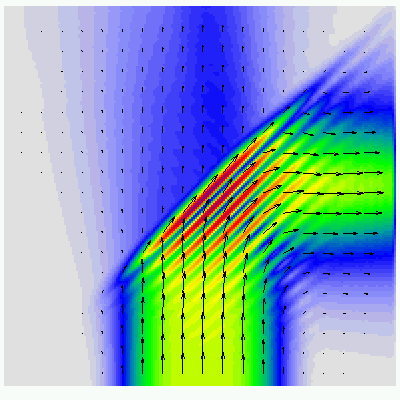
\includegraphics[width=0.8\textwidth]{fig2_06a}\\
\scriptsize{Нарушенное полное внутреннее отражение (frustrated total internal reflection, FTIR)}
\end{figure}
\end{column}
\hfill
\begin{column}[c]{6.5cm}
\centering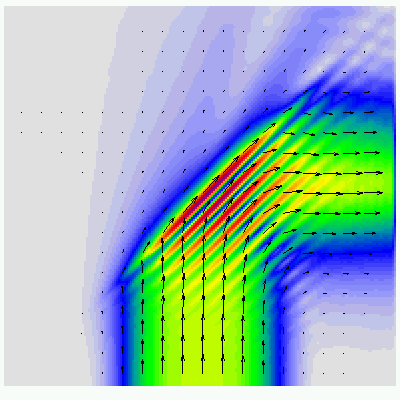
\includegraphics[width=0.8\textwidth]{fig2_06b}\\
\scriptsize{Полное внутреннее отражение (total internal reflection, TIR)}
\end{column}
\end{columns}

Попробуем внести в область ПВО еще одну среду, но такую чтобы на границе с ней мы бы находились вне зоны ПВО. Тогда в этой третьей среде мы получим вновь обыкновенную распространяющуюся волну, способную добраться до детектора, но уже несущую на себе "<отпечаток"> взаимодействия с ЭВ.

\end{frame}

\begin{frame}{Итак, что на детекторе?}

\begin{columns}[c]
\column{6.5cm}
\begin{center}
\begin{figure}
\centering
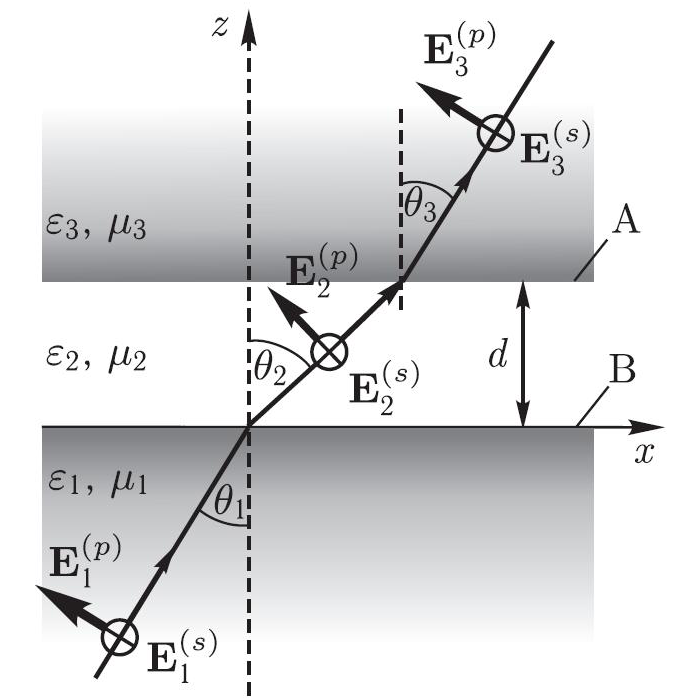
\includegraphics[width=0.9 \textwidth]{fig2_05}
\\\scriptsize{Схема НПВО}
\end{figure}
\end{center}
 
 \column{6.5cm}
\begin{center}
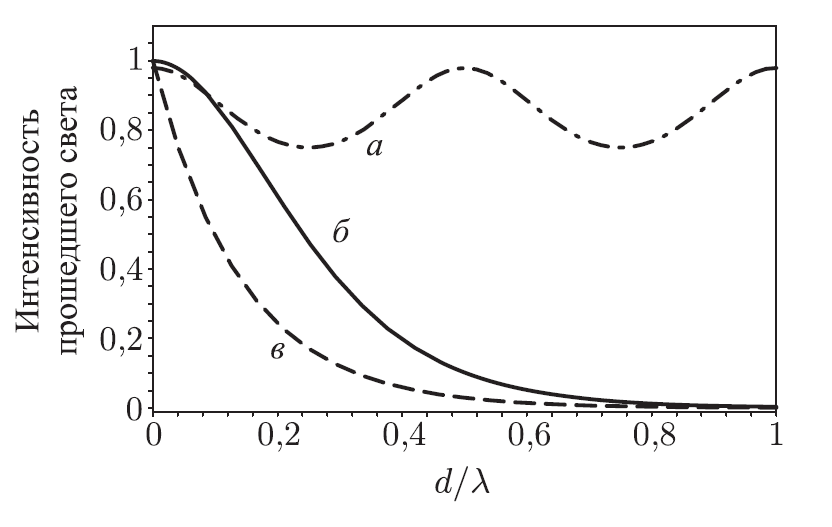
\includegraphics[width=0.9\textwidth]{fig2_14}
\\\scriptsize{Зависимость интенсивности поля на детекторе от величины зазора}
\end{center}
\end{columns}

Интенсивность поля на детекторе является монотонной (т.е. однгозначной!) функицей величины зазора. Это значит, что по карте интенсиновсти мы можем строить, например, карту поверхности (т.е. прописывать ее профиль).

\end{frame}

\begin{frame}[fragile]
\frametitle{1928 г. - рождение идеи ближнепольного микроскопа}
\begin{columns}[c]
\column{7cm}

Ирландский ученый \textcolor{red}{Эдвард Хатчинсон Синг (Edward Hutchinson Synge) в 1928 г.} предложил устройство, содержащее в себе две главные идеи реализованного полвека спустя микроскопа: (1) очень малое отверстие (или, наоборот, выступающую неоднородность, т.е. зонд) и (2) его сканирование над поверхностью образца. Вплоть до мельчайших подробностей он описал устройство зонда в двух своих пророческих работах 1928 и 1932 годов. Для удержания апертуры на небольшом расстоянии от образца Синг предложил использовать пьезоэлектрический преобразователь.

\column{5cm}
\begin{center}
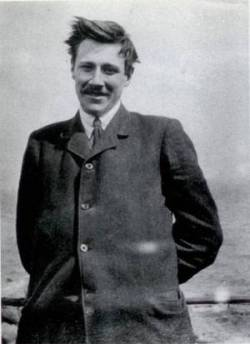
\includegraphics[width=0.9\textwidth]{ehs}
\\\scriptsize{Эдвард Хатчинсон Синг}
\end{center}
\end{columns}

\small{Он даже сделал оценку, что для перемещения на 5 $\mu$м потребуется приложить напряжение 250 В. Удивительно, что эта оценка почти идеально совпала величинами, ставшими реальными через  полвека.}
\end{frame}


\begin{frame}[fragile]
\frametitle{Переписка Э. Синга с А. Эйнштейном }

В апреле и мае 1928 года Эдвард Синг пишет несколько писем Альберту Эйнштейну. Эйнштейн отвечает
ему благожелательно и поддерживает в вопросе публикации, но констатирует:
\begin{center}
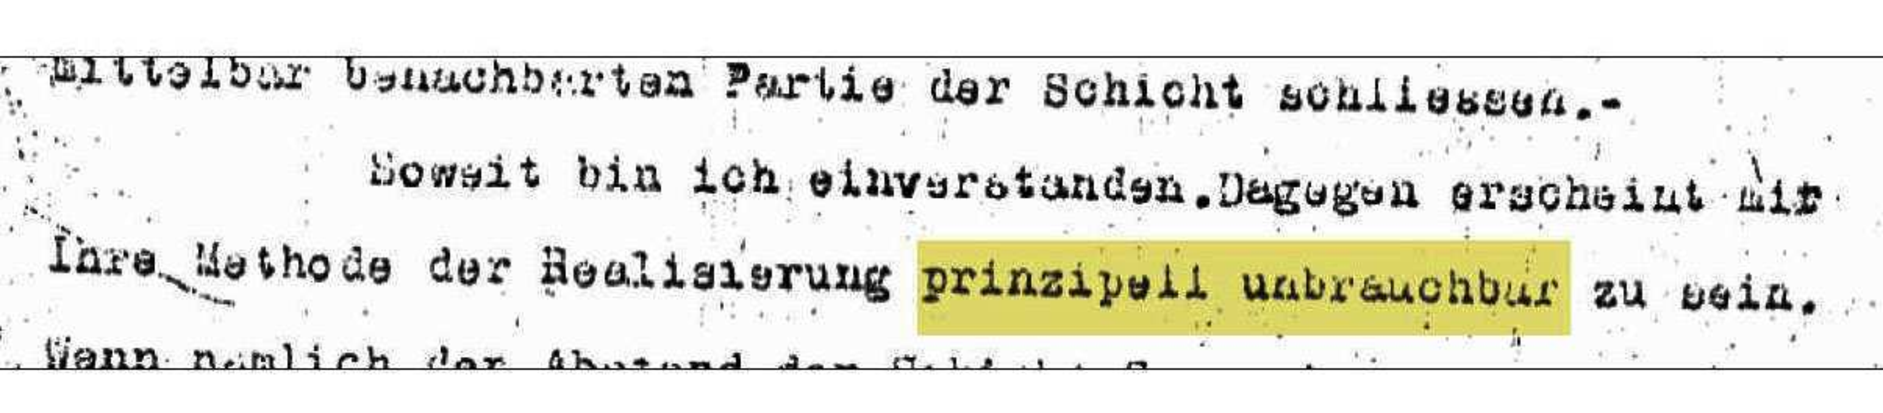
\includegraphics[scale=0.3]{eins}
\end{center}
В августе Синг сообщает Эйнштейну, что разработал схему устройства для рентгеновского диапазона и
ему даже удалось связаться с У. Брэггом, но тот не смог дать какой-нибудь удовлетворительный ответ.
Никакого свидетельства о новых ответах Эйнштейна обнаружить не удается. В 1936 году Синга постигло
умственное расстройство и остаток своих дней он провел в специальной лечебнице в Дублине. По иронии судьбы практически в точности прибор Синга был запатентован компанией Fuiji Xerox Co. в 2001 г. за авторством Kiichi Ueyanagi.

\end{frame}

\begin{frame}[fragile]
\frametitle{Факсимиле статьи Эдварда Синга}

\begin{center}
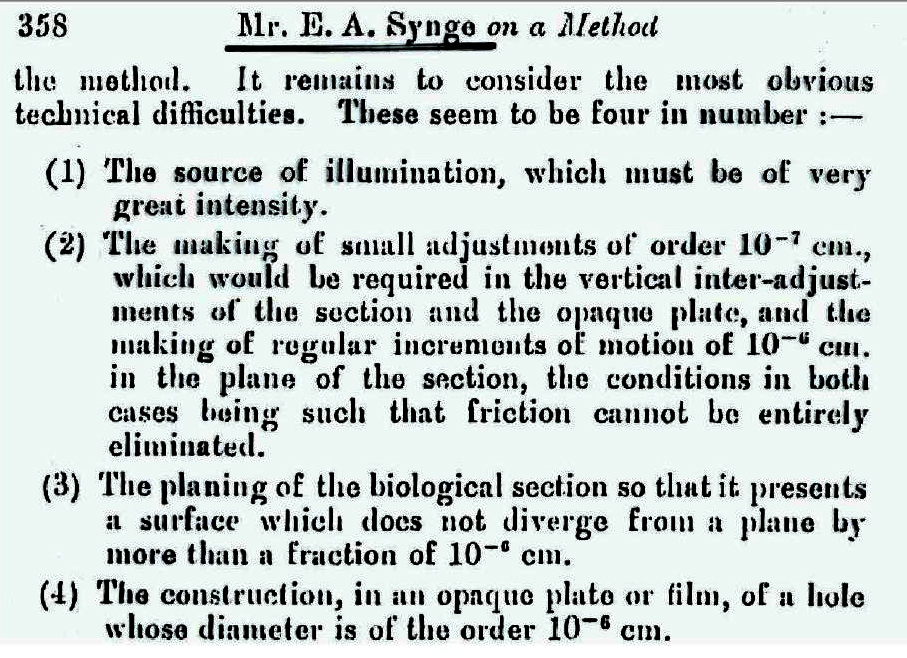
\includegraphics[scale=0.4]{synge}
\end{center}

\end{frame}


\begin{frame}[fragile]
\frametitle{Принцип сканирования}

\begin{columns}[c]
\column{6cm}
\begin{center}
В 1984 году Поль, Денк и Ланц получили первые оптические скановые траектории, и
предложили называть возникшую новую науку \underline{оптической стетоскопией}.
\end{center}
 
 \column{6cm}
\begin{center}

\includegraphics[width=0.9\textwidth]{doctor}
\end{center}
\end{columns}



В чем была идея? В своей статье они пишут: "<Например, знакомый всем медицинский стетоскоп, которым
пользуется доктор, позволяет определить место расположения сердца с точностью в пределах 10 см,
путем перемещения стетоскопа по груди пациента и слушанию биения его сердца. 

Предполагая, что звуковая частота составляет 30\,--\,100 Гц, что отвечает длине волны 100 м, мы получим, что разрешающая способность стетоскопа примерно $\lambda/1000$!">

\end{frame}


\begin{frame}[fragile]
\frametitle{Физический принцип превышения порога}
\begin{center}
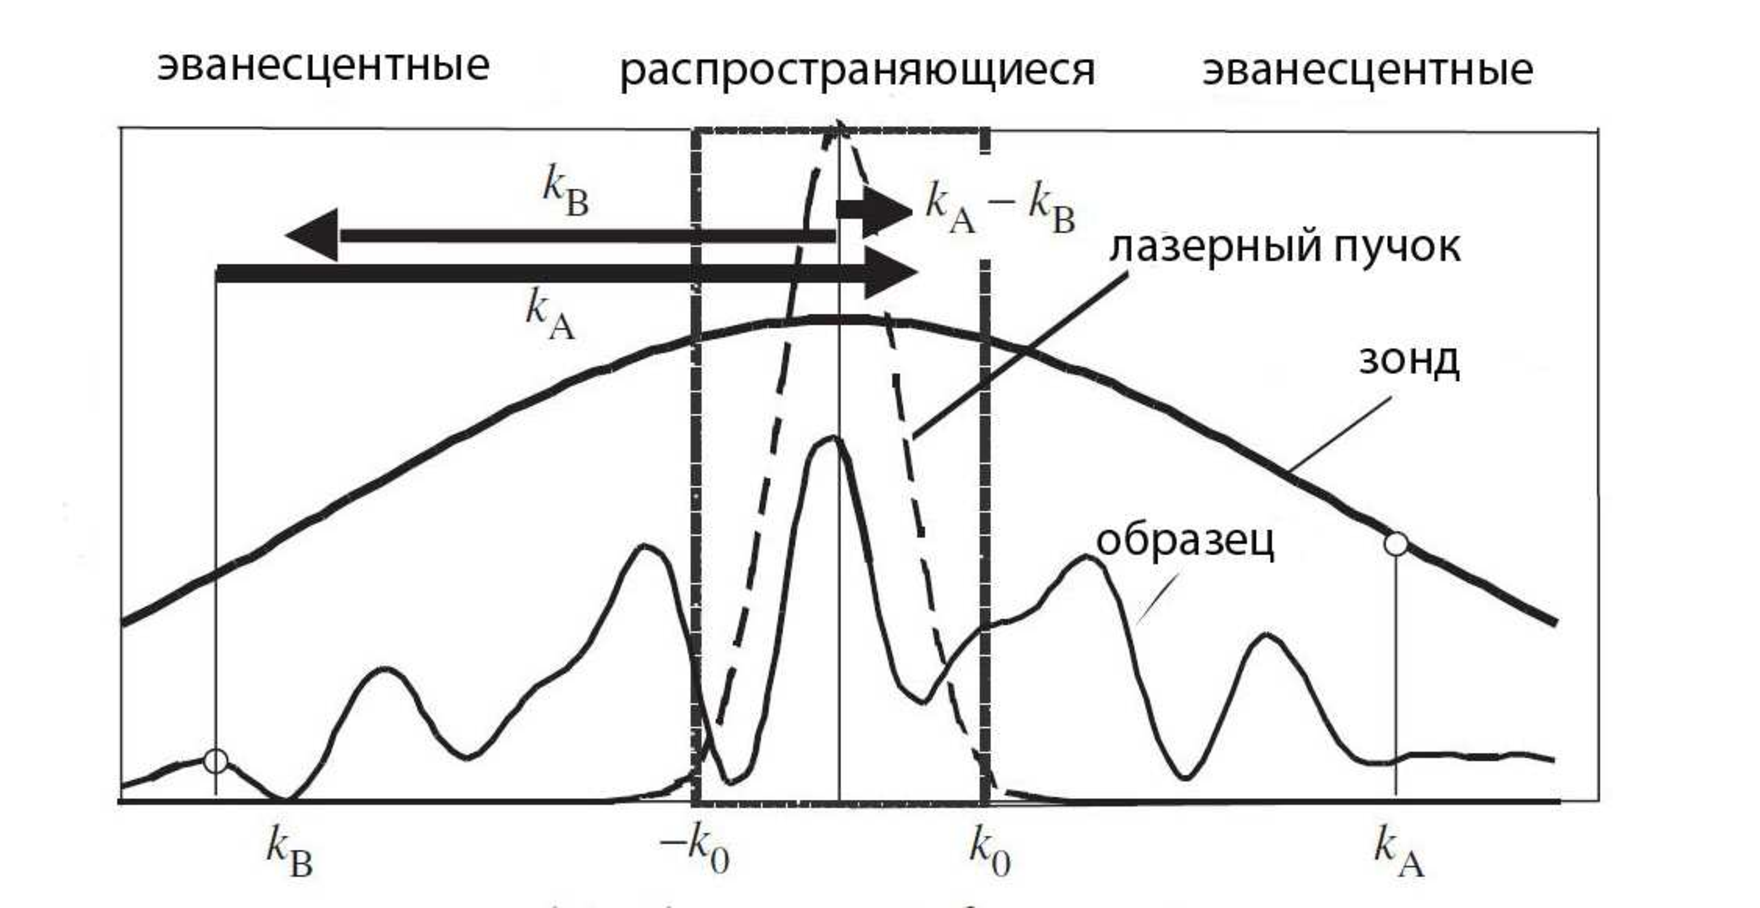
\includegraphics[scale=0.35]{evanescent}
\end{center}

Именно поэтому критерий Аббе - это постулат, родственный принципу неопределенности Гайзенберга. Не имеет эванесцентной компоненты только плоская волна в бесконечном однородном пространстве. А чтобы получить побольше область ЭВ, мы должны посильнее ужать наше поле.

\end{frame}

\begin{frame}[fragile]
\frametitle{Физический принцип превышения порога}

\begin{equation*}
\vec E (\vec r, t) = \vec E(k_x, k_y) \times \exp (\imath k_z z+ \imath k_x x+\imath k_y y - \imath
\omega t)
\end{equation*}

\begin{equation*}
k_z = +\sqrt{\omega^2 c^{-2} - k_x^2 - k_y^2},\quad \omega^2 c^{-2} > k_x^2 + k_y^2
\end{equation*}
распространяющиеся волны

\begin{equation*}
k_z = +\sqrt{\omega^2 c^{-2} - k_x^2 - k_y^2},\quad \omega^2 c^{-2} < k_x^2 + k_y^2
\end{equation*}
эванесцентные волны

Предельное разрешение: $\Delta \approx \frac{2 \pi}{k_{max}} = \lambda$

\textcolor{red}{Два выхода}

1. Детектировать эванесцентное поле.

2. Взять среду с отрицательным преломлением, для которой
\begin{equation*}
k_z = -\sqrt{\omega^2 c^{-2} - k_x^2 - k_y^2}.
\end{equation*}

\end{frame}

\begin{frame}[fragile]
\frametitle{Принципиальная схема апертурного SNOM}

\begin{center}
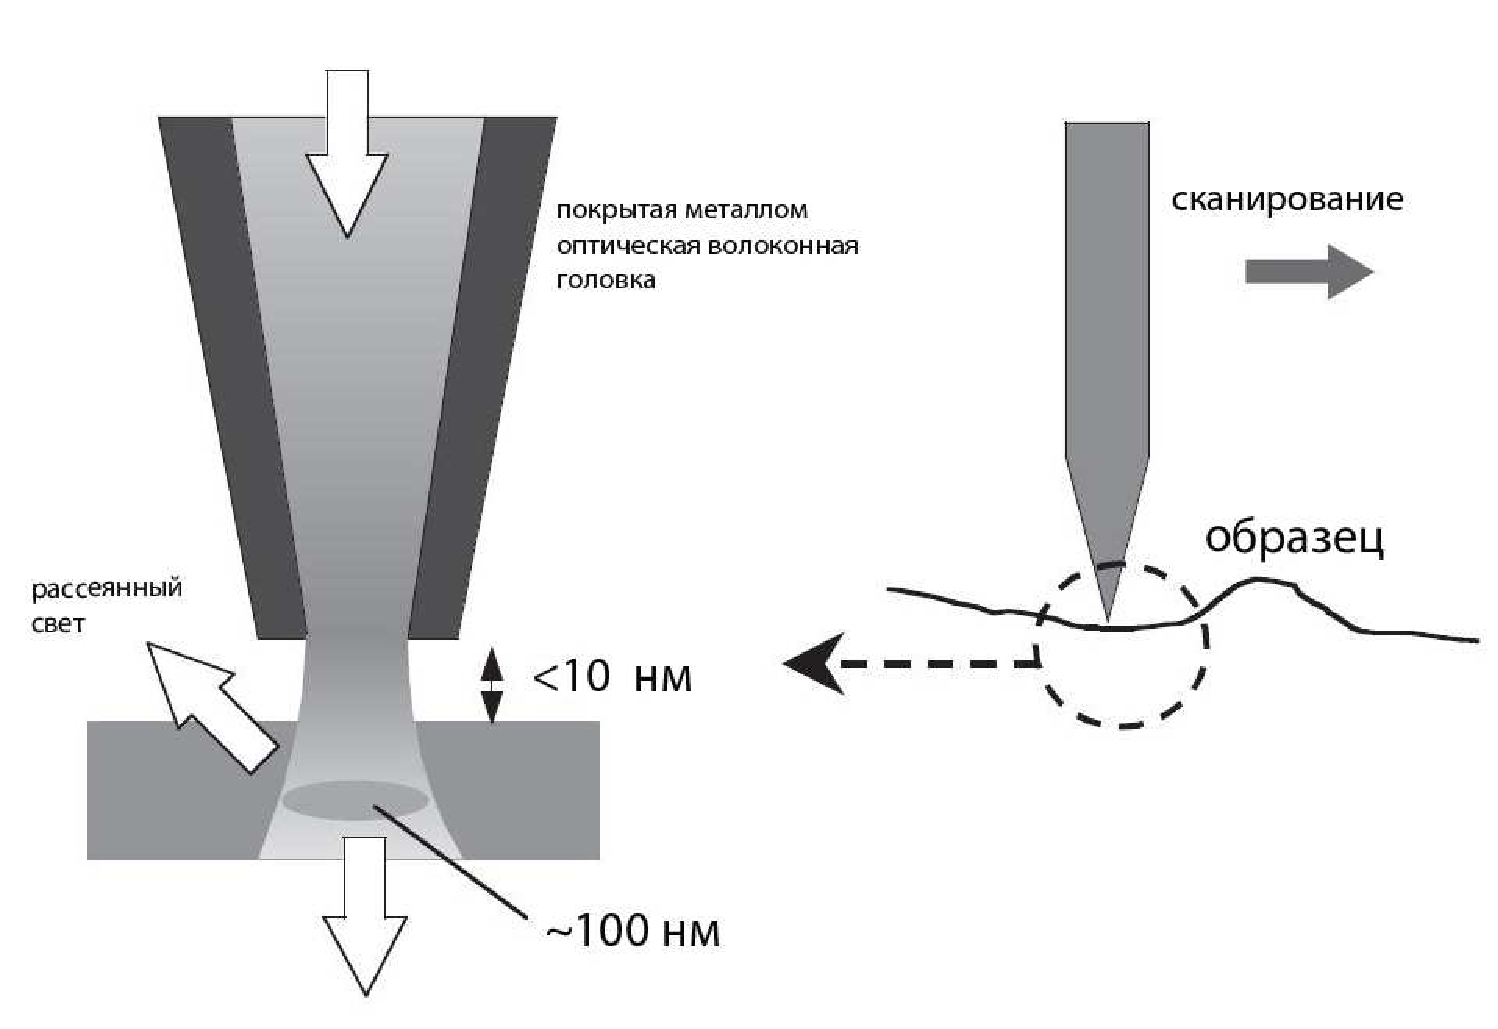
\includegraphics[scale=0.3]{apert}
\end{center}

Предельное разрешение определяется технологией сведения волокна
на конус, покрытия его металлом или пробивки отверстий, и
составляет $50$ нм.

\end{frame}

\begin{frame}[fragile]
\frametitle{Как выглядит апертурный SNOM}

\begin{center}
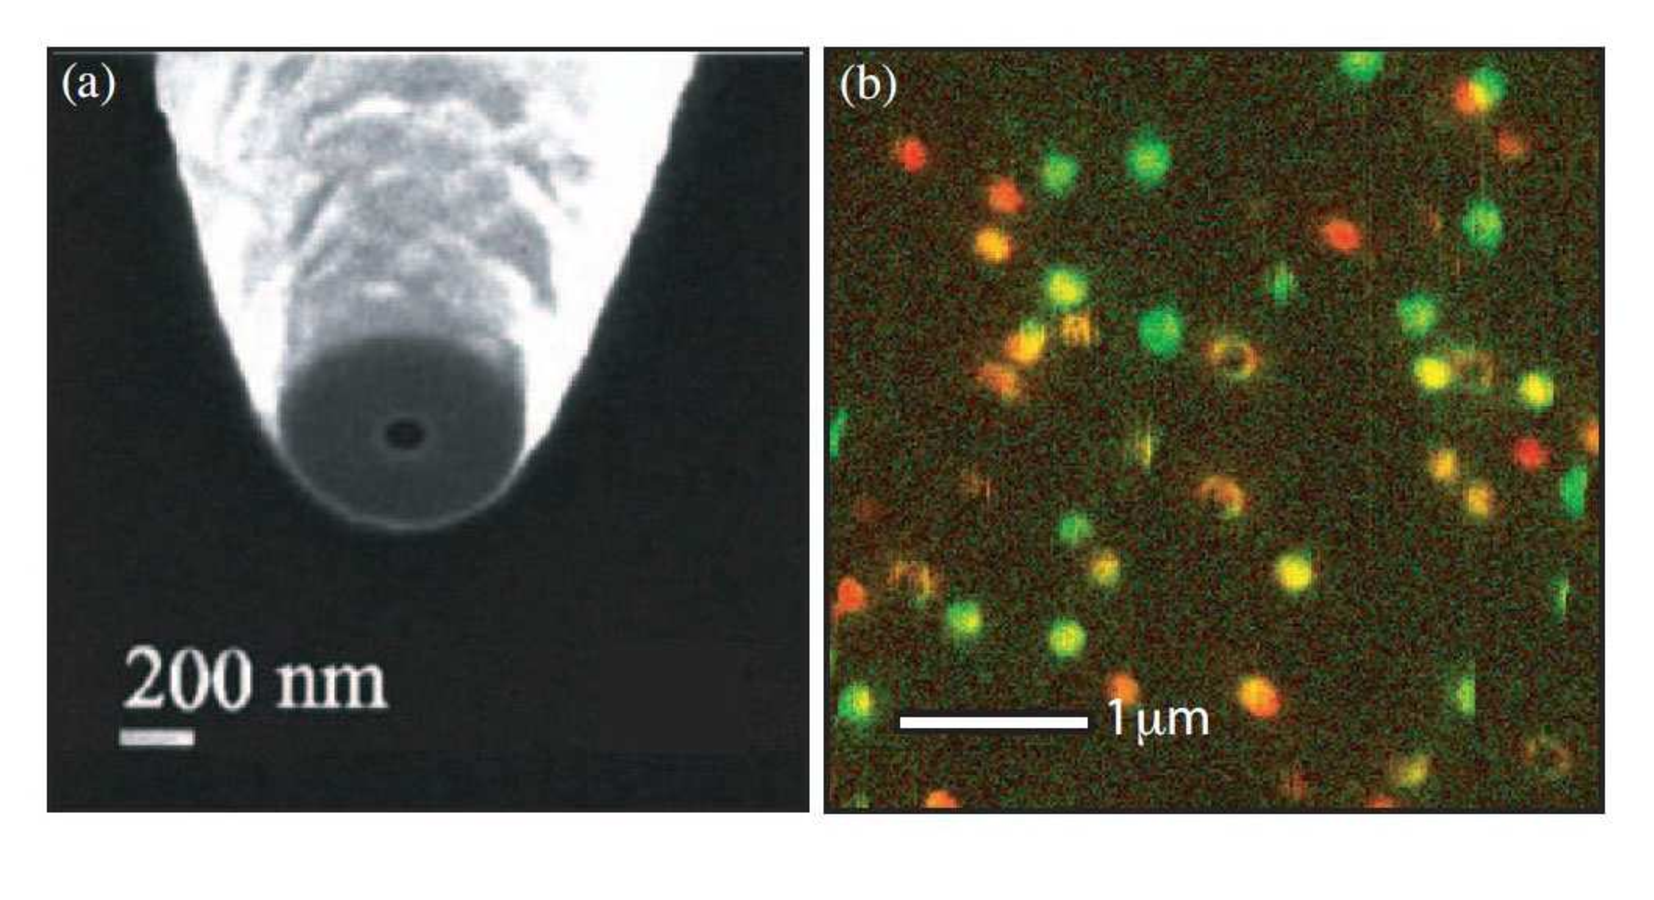
\includegraphics[scale=0.3]{probe}
\end{center}

Полученное с помощью сканирующего электронного микроскопа изображение апертурного зонда,
изготовленного путем отрезания кончика конического волокна, покрытого металлом при помощи ионной
бомбардировки  (сфокусированного ионного пучка).

\end{frame}

\begin{frame}[fragile]
\frametitle{Принципиальная схема безапертурного SNOM}

\begin{center}
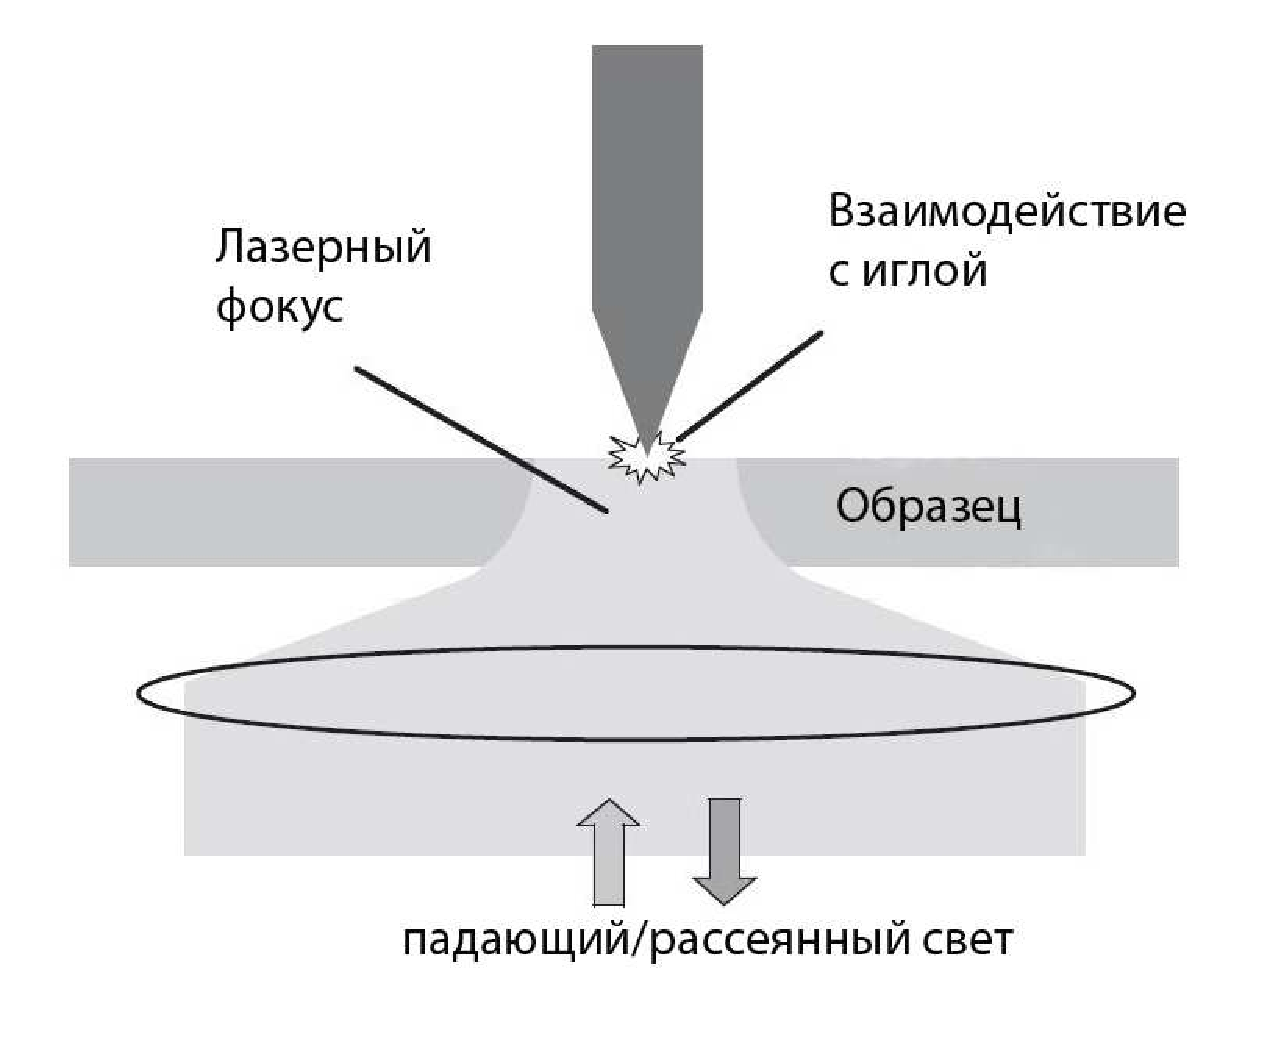
\includegraphics[scale=0.3]{apertless}
\end{center}

1. Эффект громоотвода

2. Наночастица или флуоресцентная молекула, прикрепленная к зонду

\end{frame}


\begin{frame}{Электростатическое решение задачи о тонком коническом острие}
\begin{columns}[c]
\column{4cm}
\begin{center}
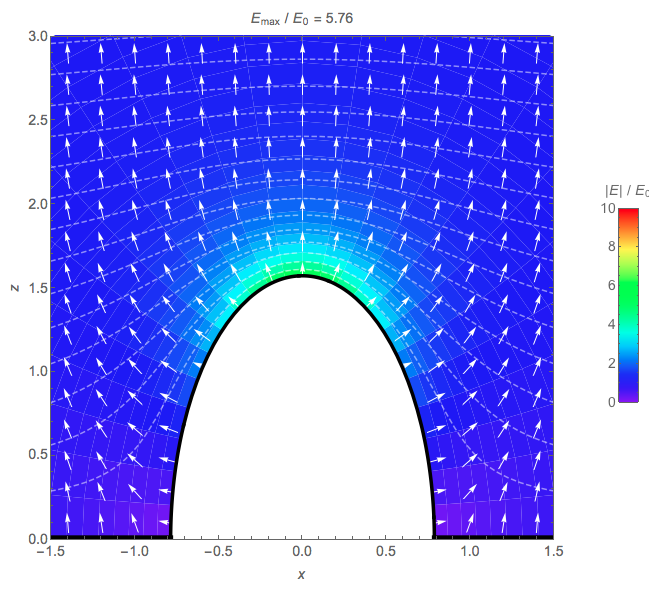
\includegraphics[width=\textwidth]{stat3}
 \end{center}
\column{4cm}
\begin{center}
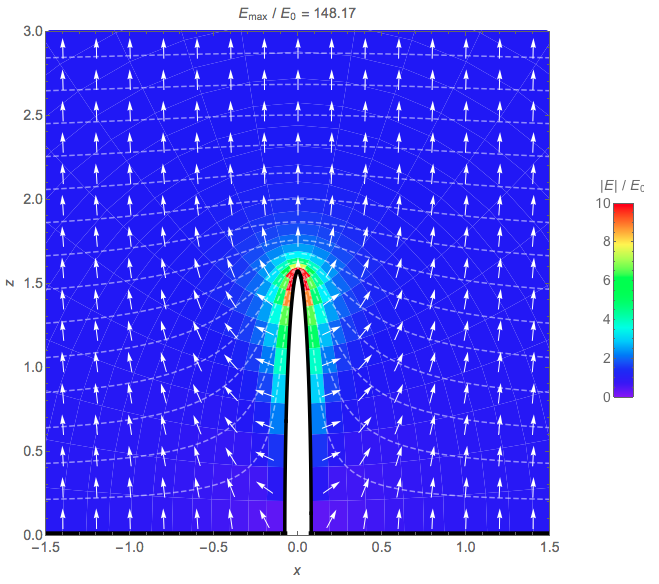
\includegraphics[width=\textwidth]{stat1}
 \end{center}
 \column{4cm}
\begin{center}
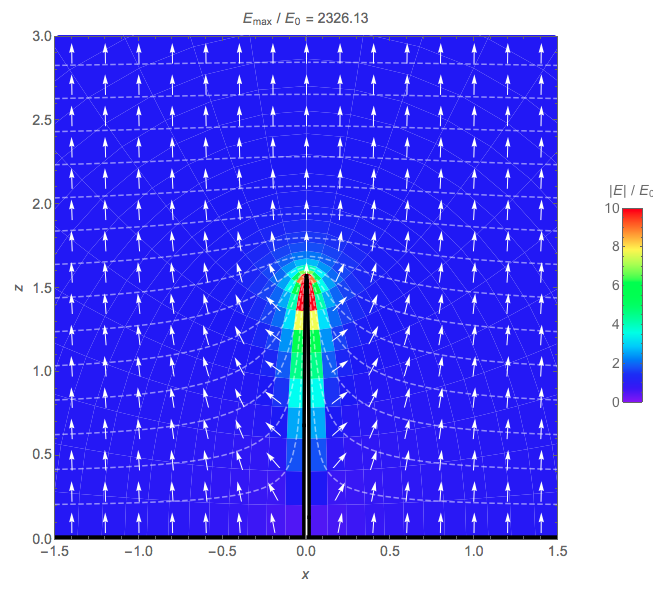
\includegraphics[width=\textwidth]{stat2}
\end{center}
\end{columns}
\scriptsize{Ландау, Лифшиц, "<Электродинамика сплошных сред">, т.VIII, 1992, с. 33 или А. Стреттон, "<Теория электромагнетизма">}
\begin{equation*}
\varphi = \varphi_0 + \varphi_1 = -a E_0 \cosh\xi\cos\eta\left(1-{\int_\xi^\infty d\xi \sinh^{-1}\xi\cosh^{-2}\xi}/{\int_{\xi_0}^\infty d\xi \sinh^{-1}\xi\cosh^{-2}\xi}\right)
\end{equation*}

\end{frame}

\begin{frame}{Плазмон и Поляритон}

\begin{columns}
\column{5cm}
{\small \textcolor{red}{Поляритон} - это связанная волна света и некоторого возбуждения в веществе. Таким возбуждением может быть плазмон.

\textcolor{red}{Плазмон} - это явление связанных колебаний электронной плотности в веществе. Если это продольные колебания, то они называются объемными плазмонами. На поверхности металла и диэлектрика можно возбудить и другой вид колебаний, поперечных. Такие колебания называются \textcolor{red}{поверхностными плазмон-поляритонами}.}
\column{7cm}
\begin{center}
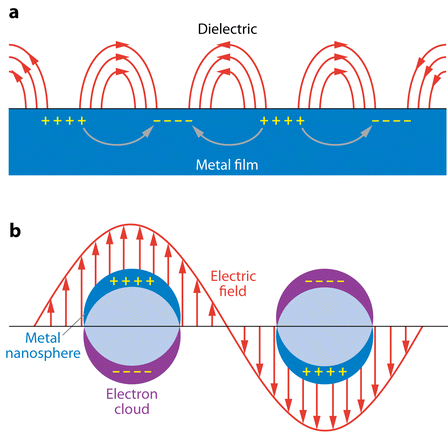
\includegraphics[width=0.9\textwidth]{spp_nanosphere}
\end{center}
\end{columns}
\end{frame}


\begin{frame}[fragile]
\frametitle{Дисперсионная кривая ППП}

\begin{center}
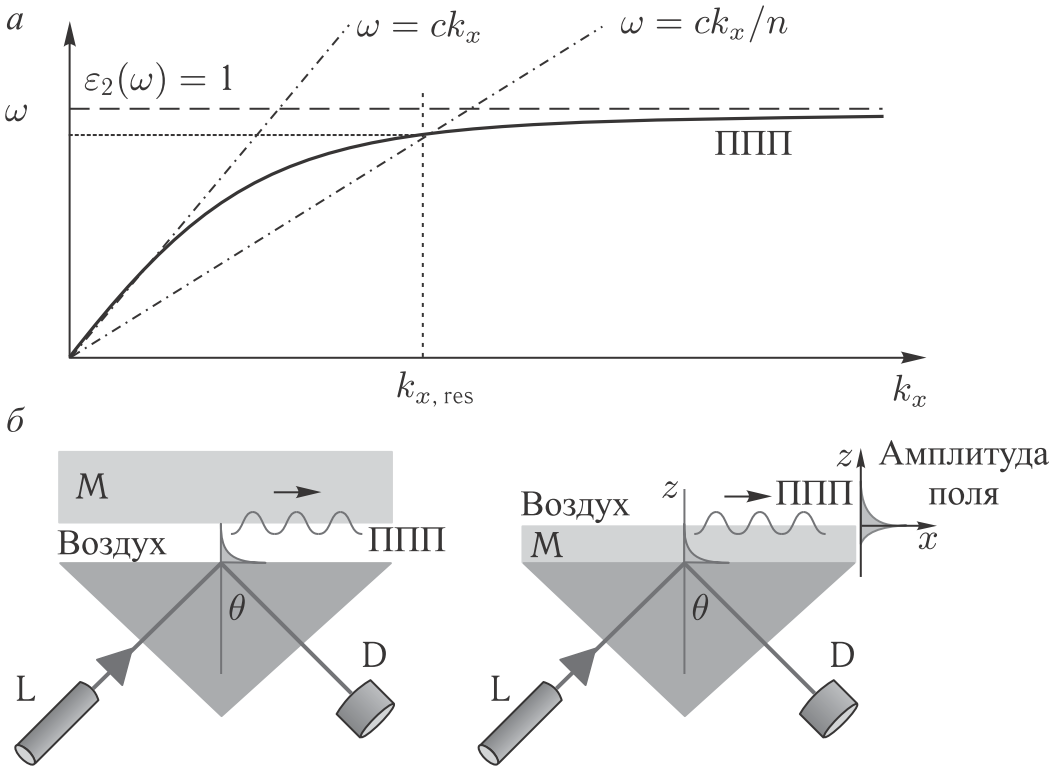
\includegraphics[width=0.9\textwidth]{plasmon}
\end{center}

\end{frame}

\begin{frame}{Фотонные кристаллы и метаматериалы}
\begin{center}
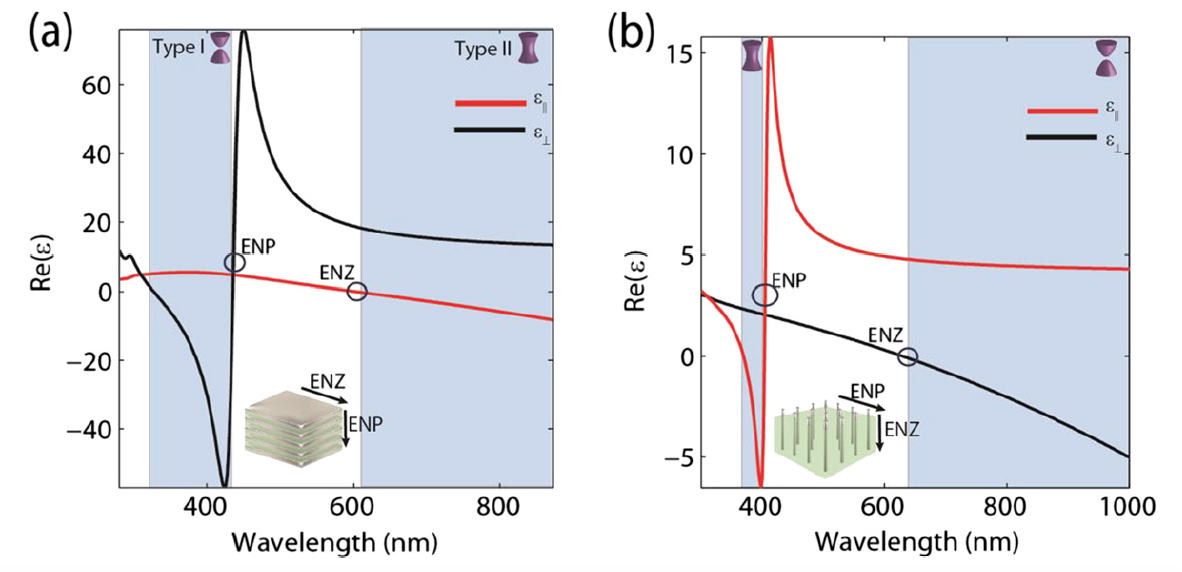
\includegraphics[width=\textwidth]{disp1}
 \end{center}
\end{frame}

\begin{frame}{Фотонные кристаллы и метаматериалы}
\begin{center}
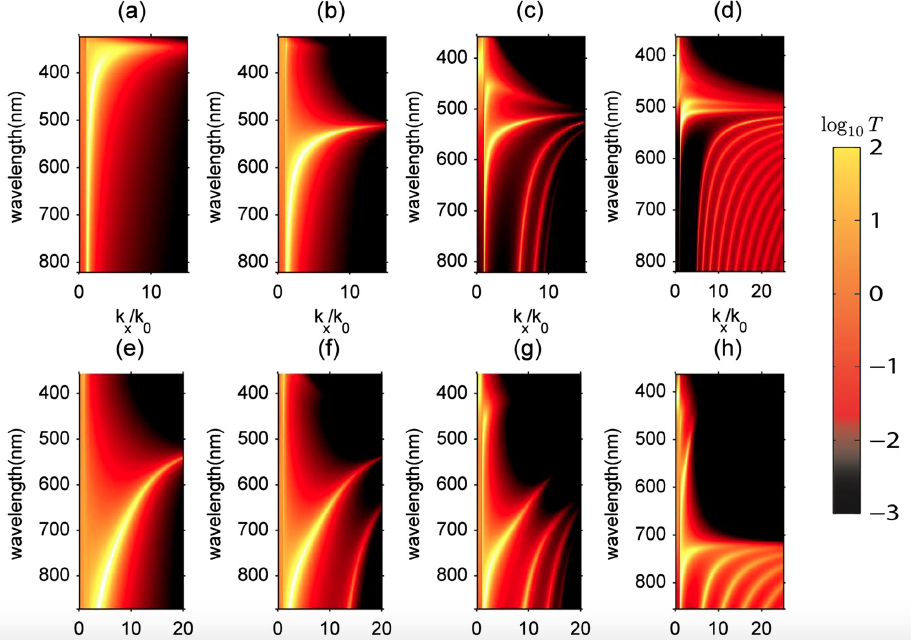
\includegraphics[width=\textwidth]{disp}
 \end{center}
\end{frame}

\begin{frame}[fragile]
\frametitle{"<Идеальная линза">: микроскопия на основе метаматериалов}

\begin{columns}[c]

\column{4cm}
\begin{center}
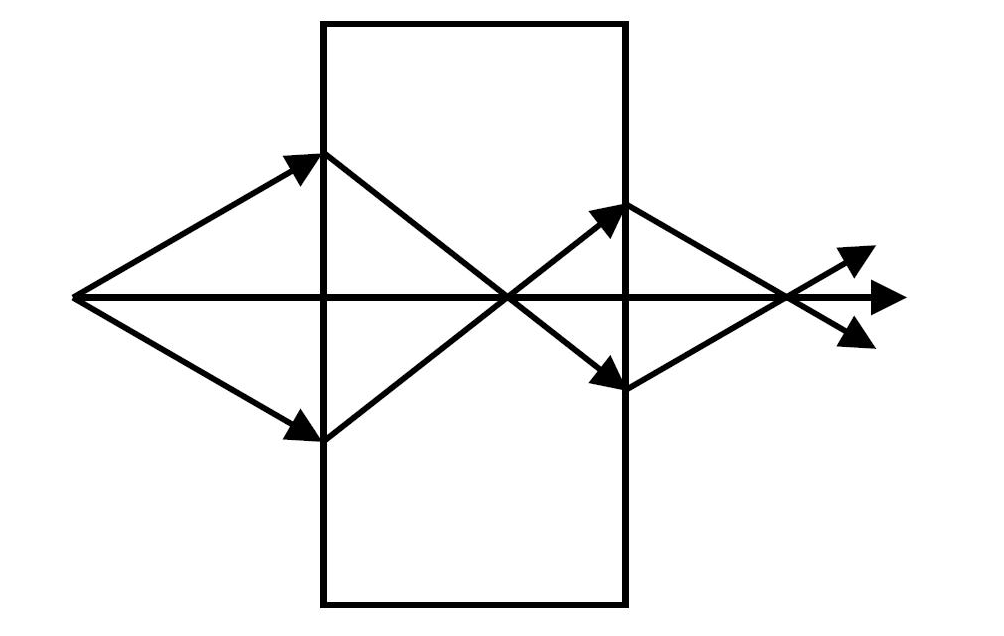
\includegraphics[width=0.9\textwidth]{pendry1}
\end{center}
\column{4cm}
\begin{center}
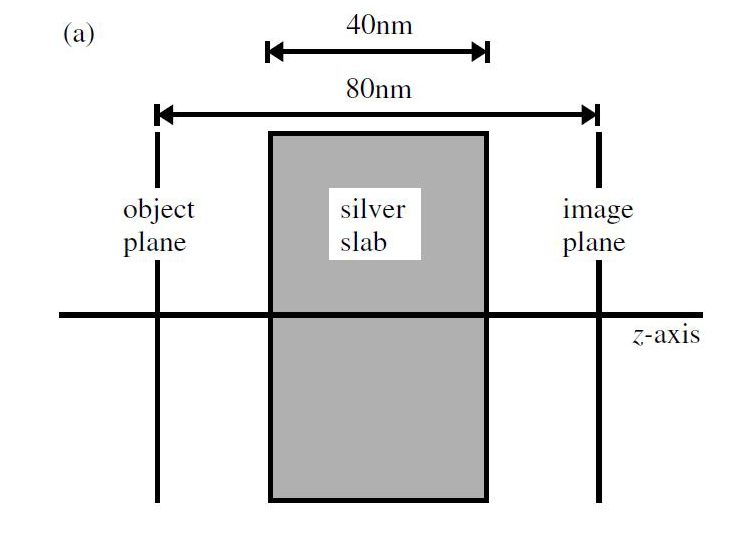
\includegraphics[width=0.9\textwidth]{pendry2}
\end{center}
\column{4cm}
\begin{center}
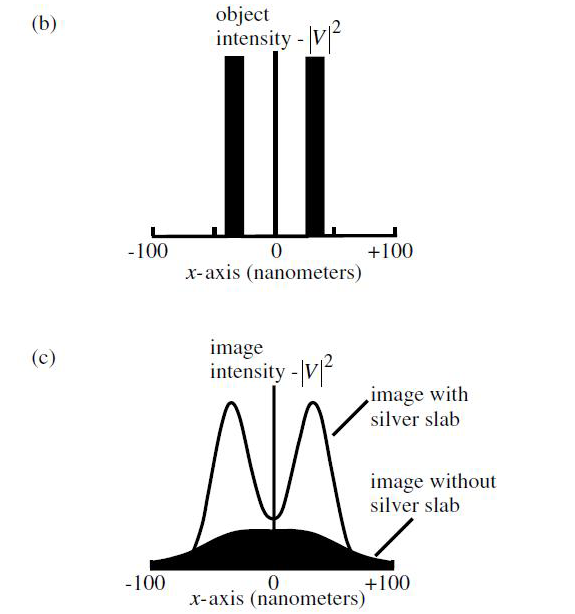
\includegraphics[width=0.9\textwidth]{pendry3}
\end{center}
\end{columns}

\begin{center}
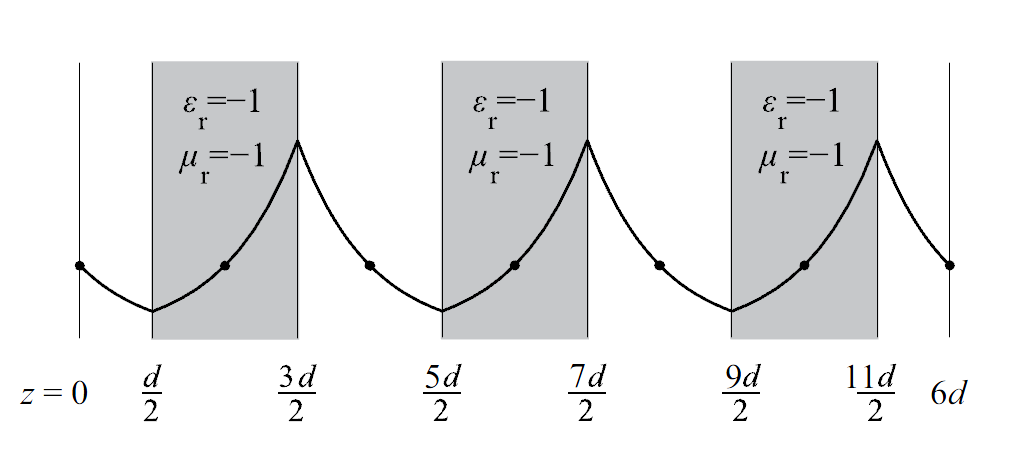
\includegraphics[width=0.7\textwidth]{neg_ref_40b}
\end{center}

\end{frame}

\begin{frame}[fragile]
\frametitle{Линзы на основе нанорешеток: пример группа Н. Желудева}

\begin{columns}[c]

\column{6cm}
\begin{center}
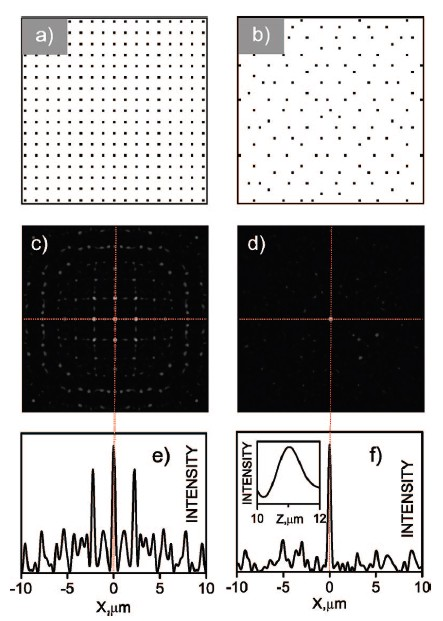
\includegraphics[width=0.9\textwidth]{array_lense}
\end{center}
\column{6cm}
\begin{center}
\includegraphics[width=0.9\textwidth]{array_lense1}
\end{center}
\end{columns}

\begin{center}
\includegraphics[width=0.7\textwidth]{neg_ref_40b}
\end{center}

\end{frame}


\begin{frame}{Фёрстеровский перенос энергии}

\begin{columns}[c]

\column{5cm}

Если два диполя находятся друг относительно друга на расстоянии меньше длины волны возможных излучательных переходов, то излучательная передача энергии от одного к другому невозможна. Зато возможен безызлучательный перенос. По \textcolor{red}{механизму Фёрстера} (1, электростатический) и по механизму Декстера (2, обменный, перекрытие молекулярных орбиталей). 

\column{7cm}
\begin{center}
\includegraphics[width=0.7\textwidth]{fret}
\end{center}
\end{columns}

\textcolor{red}{Ферстеровский радиус} порядка нескольких десятком нанометров, скорость спадает как $r^{-6}$. Это позволило использовать его в микроскопии.


\end{frame}


\begin{frame}{Сдвиг Гуса-Хенхен}

\begin{columns}[c]

\column{6.5cm}
\begin{center}
\includegraphics[width=0.8\textwidth]{ghsh}
\end{center}
 

\column{6.5cm}
\begin{center}
\includegraphics[width=0.9\textwidth]{goos-hanchen_shift}
\end{center}
\end{columns}

В области ПВО существует еще одно интересное явление - сдвиг пучка по отношению к направлению геометрической оптики (сдвиг Гуса-Хенхен, 1947 г.). Благодаря чувствительности этого явления к области ПВО, мы можем построить сенсорное устройство, которое будет работать в области т.н. отстроенного ПВО (attenuated total internal reflection, ATIR). Кроме того, мы можем усилить сдвиг пучка, возбуждая плазмон-поляритон или фонон-поляритон, и тогда величина его достигнет нескольких десятков длин волн, что мы сможем прекрасно отследить!

\end{frame}


\section{Дальнепольные методы в современной микроскопии}


\begin{frame}[fragile]
\frametitle{1961 г. - рождение идеи конфокальной микроскопии}
\begin{figure}
\centering
\includegraphics[width=0.6\textwidth]{confocal}
\end{figure}

\end{frame}

\begin{frame}{Работы группы Штефана Хилла}

\begin{columns}[c] \column{6.5cm}

\begin{center}
\includegraphics[width=0.9\textwidth]{STED1}
\end{center}

\column{6.5cm}
\begin{center}
\includegraphics[width=0.9\textwidth]{STED2}
\end{center}

\end{columns}

Нобелевская премия по химии, 2014 г.

\end{frame}


\begin{frame}{Иллюстрация идеи увеличения разрешения посредством насыщения}

\begin{center}
\includegraphics[width=11cm]{fig4_07f}
\end{center}

\scriptsize{(а) Схема энергетических уровней двухуровневой молекулы, скорость поглощения $\gamma_e$,
скорость спонтанного распада $\gamma_r$, скорость вынужденного испускания $\gamma_d$. (б)
Поперечные профили интенсивности для поглощения и вынужденного испускания. Нулевое значение
вынужденного испускания находится в точке максимума поля испускания. (в) Поперечный профиль
флоуресценции ($\gamma_r$), для двух различных значений параметра истощения уровня $d_p = 0$ и $d_p
= 100$. Чем больше этот параметр, тем \'{у}же пик флуоресценции.}
\end{frame}


\begin{frame}{STED+конфокальная: изображение живых клеток}

\begin{center}
\includegraphics[width=7cm]{fig4_07g}
\end{center}

Saccharomyces cerevisiae (пекарские дрожжи)

\begin{center}
\includegraphics[width=7cm]{fig4_07h}
\end{center}

Escherichia coli (кишечная палочка)

\end{frame}



\plain{}{Литература}

\begin{frame}{Литература по курсу:}

\begin{enumerate}
\item A. Zayats, D.Richards, "<Nano-Optics and Near-Field Optical Microscopy">, ARTECH HOUSE, 2009.
\item A. A. Maradudin "<Light scattering and Nanoscale Surface Roughness">, Springer, 2007.
\item Л. Новотный, Б. Хехт, "<Основы нанооптики">, Издательство ФИЗМАТЛИТ, Москва, Россия, 2009.
\item L. Solymar, E. Shamonina, "<Waves in Metamaterials">, Oxford University Press, Oxford, UK, 2009.
\item А.К. Сарычев, В.М. Шалаев "<Электродинамика метаматериалов">, Научный мир, 2011.
\item В.В. Климов "<Наноплазмоника">, ФИЗМАТЛИТ, 2010.
\item Ю.С. Кившарь, Н.Н. Розанов "<Нелинейности в периодических структурах и метаматериалах"> ФИЗМАТЛИТ, 2015.
\end{enumerate}

Материалы курса и работы магистрантов на портале:
\textcolor{red}{\underline{shoutovaoa.ru}}.


\end{frame}
\end{document}

